\documentclass[10pt]{article}
\usepackage{fancyhdr}
\usepackage{amsmath}
\usepackage{amssymb}
\usepackage{bm}
\usepackage{numprint}
\usepackage{float}
\usepackage[margin=0.75in]{geometry}
\usepackage{graphicx}
% Random packages from
% http://tex.stackexchange.com/questions/50070/landscape-figure-in-latex
% Necessary for sideways pictures
\usepackage{wrapfig}
\usepackage{lscape}
\usepackage{rotating}
\usepackage{epstopdf}
\usepackage{tablefootnote}
% for word wrap verbatim
\usepackage{listings}
\usepackage{caption}
\usepackage{multicol}
\usepackage{subfig}
\lstset{
   breaklines=true,
   basicstyle=\ttfamily}
% Include longitudinal
\graphicspath{ {../../figures/} {../../figures/longitudinal/} }
\providecommand{\e}[1]{\ensuremath{\times 10^{#1}}}

\begin{document}

\title{Cluster Analysis: Identifying Parkinson's Disease Subtypes}
\author{Jesse Mu}
\maketitle

\tableofcontents
\newpage

\begin{multicols}{2}

\section{New Content}

Section~\ref{sec:longitudinal} on longitudinal analysis; section~\ref{sec:nms30} on

\section{Preprocessing}

\subsection{Dataset Description}
951 subjects, 145 metrics, collected 15-4-2012 from Pablo Martinez Mart\'in. Only
19 features used for clustering and/or interpretation.  50 subjects with
missing values of the features to be used in clustering (brought down to 901).
It was decided to not impute the data. Data was scaled to $\mu = 0, \sigma =
1$ during clustering and modeling, then unscaled for visualization.

\subsection{Selected Features}

Combination of non-motor scale (NMS) symptoms and standard motor symptoms.
PIGD was deleted after 2015-07-16 meeting.

\begin{table}[H]
  \centering
  \begin{tabular}{l|l|l}
    Name & Type & Description \\
    \hline
    nms\_d1 & byte & cardiovascular \\
    nms\_d2 & byte & sleep/fatigue \\
    nms\_d3 & byte & mood/cognition \\
    nms\_d4 & byte & percep/hallucinations \\
    nms\_d5 & byte & attention/memory \\
    nms\_d6 & byte & gastrointestinal \\
    nms\_d7 & byte & urinary \\
    nms\_d8 & byte & sexual function \\
    nms\_d9 & byte & miscellaneous \\
    tremor & float & tremor \\
    bradykin & float & bradykinesia\tablefootnote{Impaired ability to
    adjust the body's position.} \\
    rigidity & float & rigidity \\
    axial & float & axial\tablefootnote{Issues affecting the middle of
    the body.} \\
  \end{tabular}
  \caption{Selected Features and Details}
  \label{tab:selected-features}
\end{table}

\begin{table}[H]
  \centering
  \begin{tabular}{l|l|l|l}
  Name  &       $\mu$ & $\sigma$ & min-max \\
         \hline
nms\_d1&   1.73&  3.35&   0-24 \\
nms\_d2&   8.75&  8.70&   0-48 \\
nms\_d3&   8.68& 11.55&   0-60 \\
nms\_d4&   1.64&  3.86&   0-33 \\
nms\_d5&   5.42&  7.43&   0-36 \\
nms\_d6&   5.53&  6.79&   0-36 \\
nms\_d7&   8.08&  8.94&   0-36 \\
nms\_d8&   3.52&  5.97&   0-24 \\
nms\_d9&   7.13&  7.79&   0-48 \\
tremor&   2.59&  2.58&   0-12 \\
bradykin& 2.40&  1.41&   0-6 \\
rigidity& 2.24&  1.36&   0-6 \\
axial&    3.25&  2.68&   0-12 \\
  \end{tabular}
  \caption{Descriptive Statistics}
  \label{tab:descriptive-statistics}
\end{table}

\section{Clustering}

$k$-means clustering with $k = 4$ was tried. Statistics for determining the
optimal number of clusters were used, but were generally inconclusive: results in
Figure~\ref{tab:numclus}. This probably indicates that the data is not very
well clustered. $k = 2, 3$ provided models that were too simplistic. $k = 5$
did not provide any new information, but rather just fragmented existing
groups.
\begin{table}[H]
  \centering
  \begin{tabular}{l|l}
    Criterion & Optimal $k$ \\
    \hline
    Minimum ASW & 2 \\
    BIC & 18 \\
    SSE Scree Plot & Inconclusive \\
    Gap Statistic & 4 \\
    Affinity Propagation & 8 \\%\tablefootnote{$\lambda = 0.98$, q = 0, maxits = 1000, %convits = 100} & 8 \\
    clValid stability measures & 4 \\
  \end{tabular}
  \caption{Results of various techniques for determining $k$}
  \label{tab:numclus}
\end{table}

\subsection{Decision tree}
% \begin{table}[H]
  % \centering
  % \begin{tabular}{l|l|l|l|l|l}
    % $k$ & CP\tablefootnote{Complexity Parameter} & CV Xerror\tablefootnote{10-fold cross
    % validation} & Root Feature &
    % Root Error & Figure \\
    % \hline
    % 4 & 0.0100 & 0.255 & pigd $<$ 2.5 & 0.563 & Figure~\ref{fig:kmeans-dtree-4} \\
  % \end{tabular}
  % \caption{$k$-kmeans decision trees statistics}
  % \label{tab:k-means-dtrees}
% \end{table}

Decision tree for $k = 4$ created via recursive partitioning is available in
Figure~\ref{fig:kmeans-dtree-4}. More discussion about the decision tree is
located in Section~\ref{feature-importance}.

\begin{figure}[H]
  \centering
  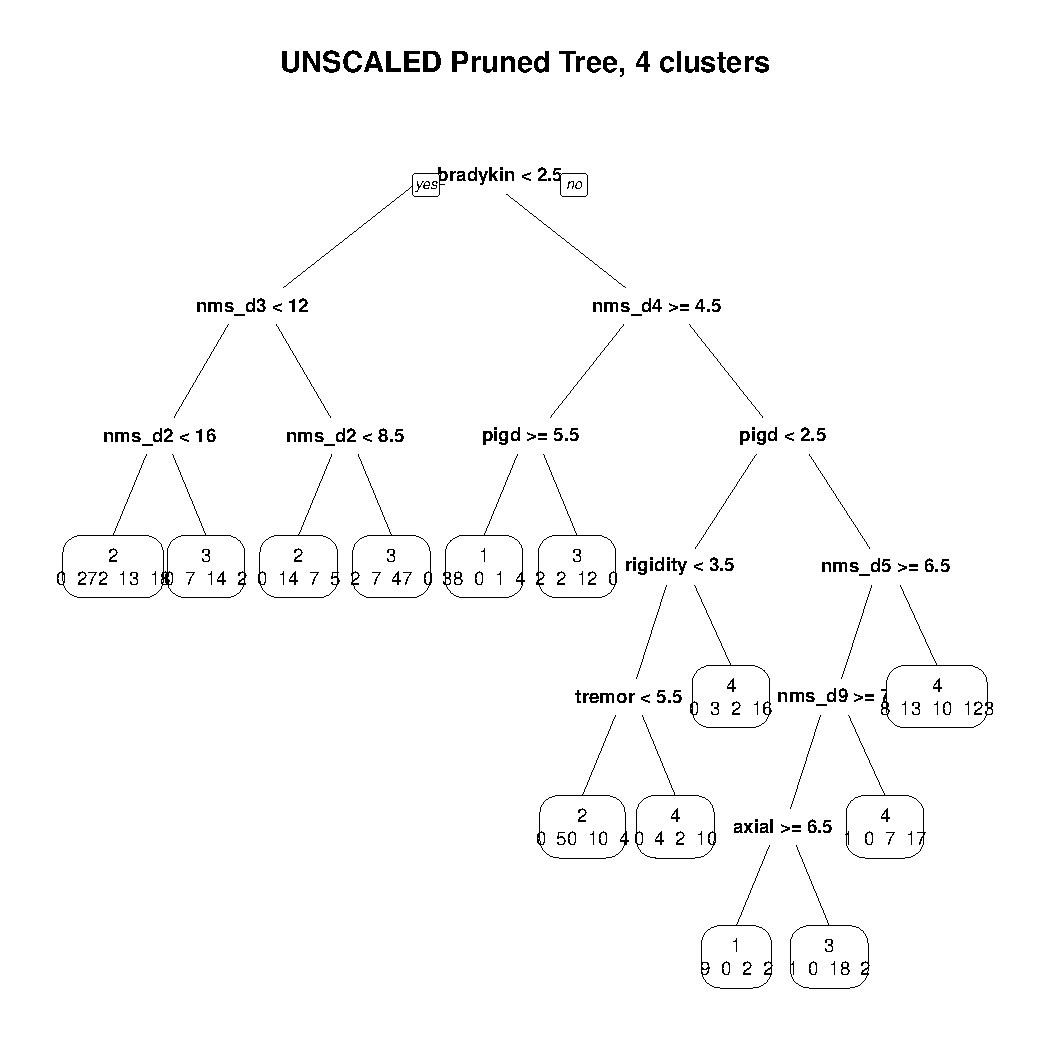
\includegraphics[width=\linewidth]{dtree-kmeans-pruned-unscaled-4.pdf}
  \caption{Decision Tree from $k$-means clustering, 4 clusters}
  \label{fig:kmeans-dtree-4}
\end{figure}

\subsection{Interpretation of Clusters}

\subsubsection{Cluster summaries}

Available in Figure~\ref{fig:kmeans-summaries-4}. Error bar is standard error.

\begin{figure*}[t]
  \centering
  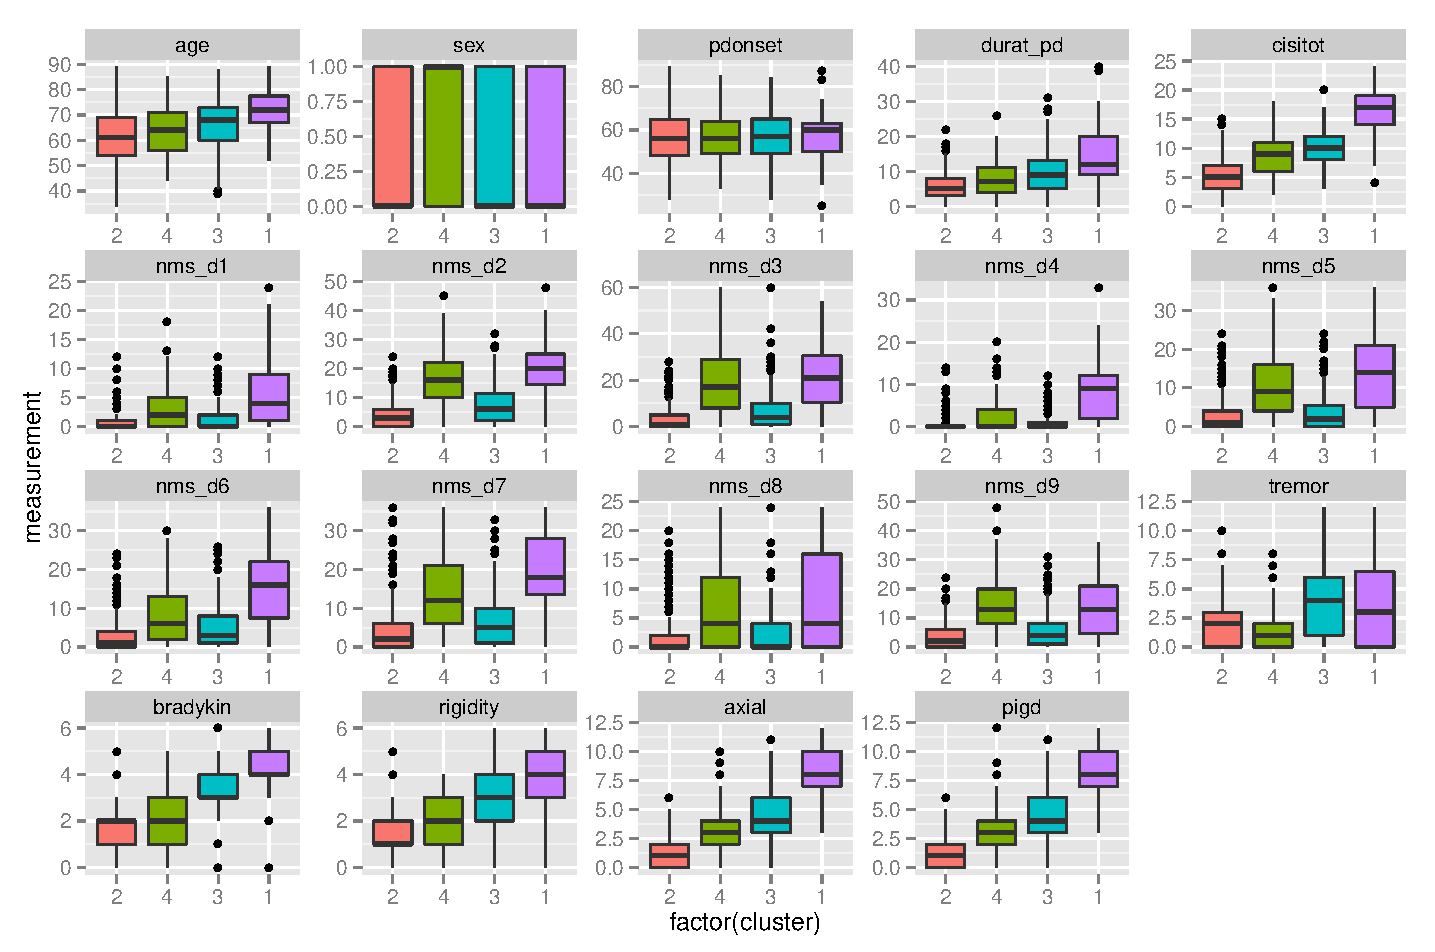
\includegraphics[width=\linewidth]{kmeans-summaries-4.pdf}
  \caption{Cluster Summaries, $k = 4$}
  \label{fig:kmeans-summaries-4}
\end{figure*}

\subsubsection{Interpretation}
$k$-means clustering ($k = 4$) found four clusters. With a brief description,
they are:

% TODO: Figure out where the cluster reordering appears in other graphs
% (kmeans, correlation) and redo those!!!
% AND THE REST OF THE PAPER
% TODO: LEVELS play a big factor - when I factor by reordering levels\dots
\begin{itemize}
  \item[1.] $(n = 406)$ Mildly affected in all domains.
  \item[2.] $(n = 189)$ Severely affected in nonmotor domains; mildly
    affected in motor domains.
  \item[3.] $(n = 221)$ Severely affected in motor domains; mildly
    affected in nonmotor domains.
  \item[4.] $(n = 88)$ Severely affected in all domains.
\end{itemize}

\subsubsection{Statistical Significance Tests, $k = 4$}
For each variable $i$ and cluster means $\mu_i^1, \mu_i^2, \mu_i^3, \mu_i^4$,
we use one-way ANOVA for multiple means and reject the null hypothesis that
$\mu_i^1 = \mu_i^2 = \mu_i^3 = \mu_i^4$ with $p < 0.05$ for every variable
except pdonset.

Post-hoc analysis using Tukey's HSD to examine statistically significant
differences between individual means is available in Table~\ref{tab:tukeyhsd}.
For brevity, only statistically insignificant relations are provided; all other
relations are significant with $p < 0.05$.

\begin{table}[H]
  \centering
  \begin{tabular}{l|l|l}
  Variable & Cluster Relation & $p$ \\
  \hline
age & 2-1 & 0.428 \\
    & 3-2 & 0.724 \\
    \hline
sex & 2-1 & 0.0918 \\
    & 3-1 & 0.216 \\
    & 4-1 & 0.827 \\
    & 4-2 & 0.849 \\
    & 4-3 & 0.161 \\
    \hline
pdonset & 2-1 & 0.859 \\
        & 3-1 & 0.700 \\
        & 4-1 & 0.305 \\
        & 3-2 & 0.370 \\
        & 4-2 & 0.147 \\
        & 4-3 & 0.803 \\
\hline
durat\_pd & 3-2 & 0.562 \\
\hline
cisitot & 3-2 & 0.522 \\
\hline
nms\_d1 & 3-1 & 0.333 \\
\hline
nms\_d4 & 3-1 & 0.557 \\
\hline
nms\_d5 & 3-1 & 0.856 \\
\hline
nms\_d8 & 3-1 & 0.122 \\
\hline
nms\_d9 & 3-1 & 0.0735 \\
       & 4-2 & 0.730 \\
\hline
tremor & 2-1 & 0.360 \\
  \end{tabular}
  \caption{Tukey's HSD Insignificant Differences}
  \label{tab:tukeyhsd}
\end{table}

\subsubsection{Feature importance}
\label{feature-importance}

Features ranked by information gain with respect to cluster are available in
Table~\ref{tab:info_gain}. Also, in the 4-cluster decision tree in
Figure~\ref{fig:kmeans-dtree-4}, features are ranked implicitly by importance
in determining clusters. We see, quite naturally, that standard measures of
motor symptoms rank very highly (ranks 1, 2, 4, 5) in information gain \emph{except}
tremor (12). Similarly, bradykinesia (1) is used as the root node of the
4-cluster decision tree, although other motor symptoms are used further down
the tree, since immediately successive motor symptom decision nodes would, due
to their determination of clusters, be redundant.

The most informative nonmotor
symptoms are nms\_d2 (sleep/fatigue) at 2, along with nms\_d3
(mood/cognition). As discussed later in Section~\ref{sub:ova} these features
become critical in one-versus-all decision trees for distinguishing various
subtypes. The importance of these nonmotor symptoms confirms the longitudinal
study by Fereshtehnejad et al. \cite{fereshtehnejad15} who cites a 3-cluster PD
subtype identification based primarily on nonmotor symptoms including cognitive
impairment, rapid eye movement sleep disorder (RBD), anxiety, and depression,
conditions that align closely with nms\_d2 and nms\_d3 as tested in this
dataset. More analysis needs to be done on whether there are parallels between
Fereshtehnejad's 3-cluster longitudinal study and the clusters found in both
this investigation and van Rooden.

Interestingly, demographic information, including durat\_pd, age, sex, and
pdonset, plays almost no role in the determination of these clusters. That the
time of onset of PD or sex is largely irrelevant provides an important negative answer to
clinically-relevant questions about the demographic sources of these different
subtypes.

\begin{table}[H]
  \centering
  \begin{tabular}{r|l|l}
    rank & variable & information gain \\
    \hline
    1 & bradykin      & 0.316 \\
    2 & rigidity      & 0.296 \\
    3 & nms\_d2      & 0.242 \\
    4 & cisitot      & 0.229 \\
    5 & axial      & 0.228 \\
    6 & nms\_d3      & 0.205 \\
    7 & nms\_d9      & 0.158 \\
    8 & nms\_d7      & 0.153 \\
    9 & nms\_d5      & 0.145 \\
    10 & nms\_d6      & 0.140 \\
    11 & nms\_d1      & 0.132 \\
    12 & tremor      & 0.109 \\
    13 & nms\_d4      & 0.107 \\
    14 & nms\_d8      & 0.100 \\
    15 & durat\_pd      & 0.0288 \\
    16 & age      & 0.0235 \\
    17 & sex      & 0.000 \\
    18 & pdonset      & 0.000 \\
  \end{tabular}
  \caption{Features ranked by information gain}
  \label{tab:info_gain}
\end{table}

\subsubsection{Correlation Plots}

The interplay between specific symptoms in each of the four clusters was
examined in Figure~\ref{fig:corrplots}. There are two points of note. The first
is that there is a higher correlation in cluster 4 (severe) between overall
severity (cisitot) and bradykinesia and rigidity, illustrated in
Figure~\ref{fig:corrxy-br}.
Second, there exists a somewhat higher correlation between
bradykinesia, rigidity, and nms\_d6 (gastrointestinal) in cluster 4,
illustrated in Figure~\ref{fig:corrxy-d6}. These differences are statistically
significant; correlation tests are located in Table~\ref{tab:cortests}. I am
unsure of the significance or proper interpretation of these results.

\begin{table*}[t]
  \centering
  \begin{tabular}{l|l|l|l}
 Cluster & Variables & 95\% CI & $p$ \\
    \hline
1 & bradykin, cisitot&[-0.0225, 0.171]&0.131 \\
  & rigidity, cisitot&[-0.000406, 0.192]&0.0510 \\
  & bradykin, nms\_d6&[-0.0634, 0.131]&0.493 \\
  & rigidity, nms\_d6&[-0.101, 0.0932]&0.934 \\
  \hline
2 & bradykin, cisitot&[0.0786, 0.351]&$0.00248^{(**)}$ \\
  & rigidity, cisitot&[-0.215, 0.069]&0.310 \\
  & bradykin, nms\_d6&[-0.152, 0.133]&0.897 \\
  & rigidity, nms\_d6&[-0.123, 0.163]&0.781 \\
  \hline
3 & bradykin, cisitot&[0.0995, 0.350]&$0.000620^{(***)}$ \\
  & rigidity, cisitot&[0.0687, 0.322]&$0.00298^{(**)}$ \\
  & bradykin, nms\_d6&[0.0350, 0.292]&$0.0134^{(*)}$ \\
  & rigidity, nms\_d6&[-0.0846, 0.179]&0.478 \\
  \hline
  4 & bradykin, cisitot&[0.454, 0.724]&${3.97\e{-10}}^{(***)}$ \\
& rigidity, cisitot&[0.375, 0.675]&${4.99\e{-08}}^{(***)}$ \\
  & bradykin, nms\_d6&[0.297, 0.624]&${2.60\e{-06}}^{(***)}$ \\
  & rigidity, nms\_d6&[0.278, 0.611]&${6.43\e{-06}}^{(***)}$ \\
  \end{tabular}
  \caption{Correlation tests. (*) $p < 0.05$, (**) $p < 0.01$, (***), $p < 0.001$}
  \label{tab:cortests}
\end{table*}

\begin{figure}[H]
  \centering
  \subfloat[][]{%
  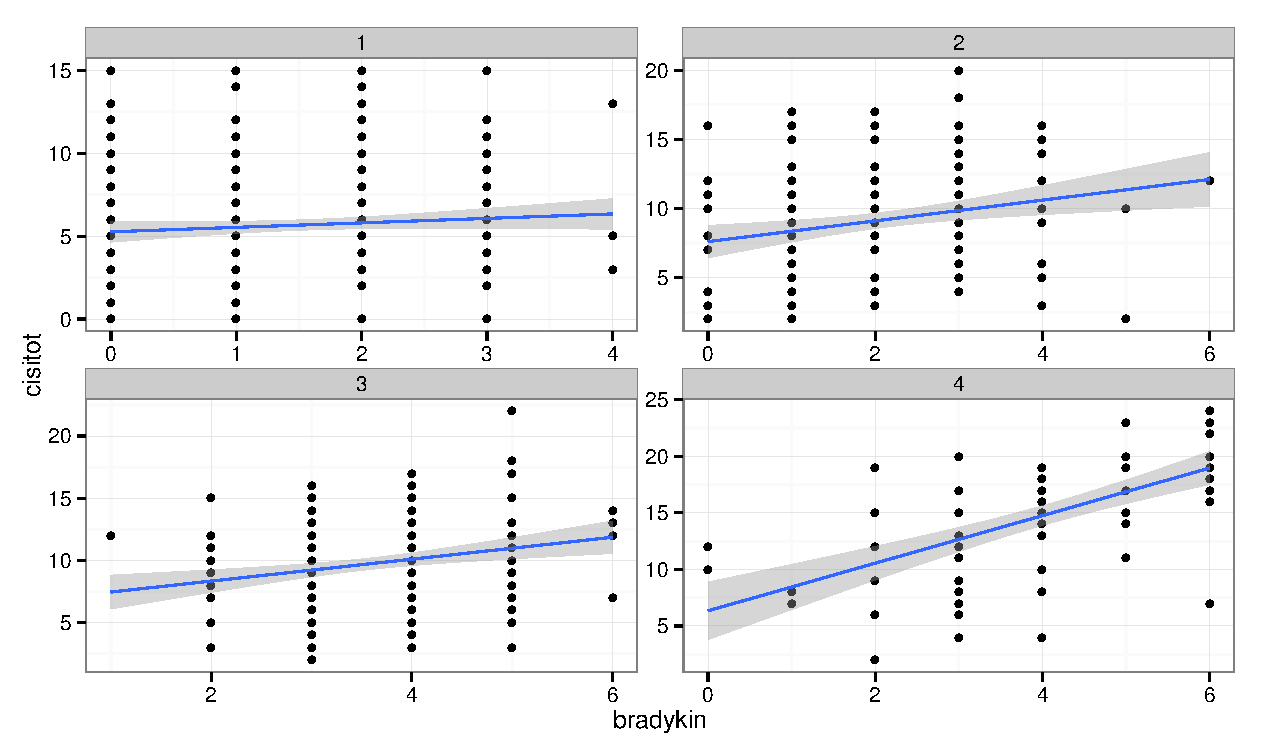
\includegraphics[clip,width=\linewidth]{bradykin-v-cisitot.pdf}
  \label{bradyv}
}

\subfloat[][]{%
  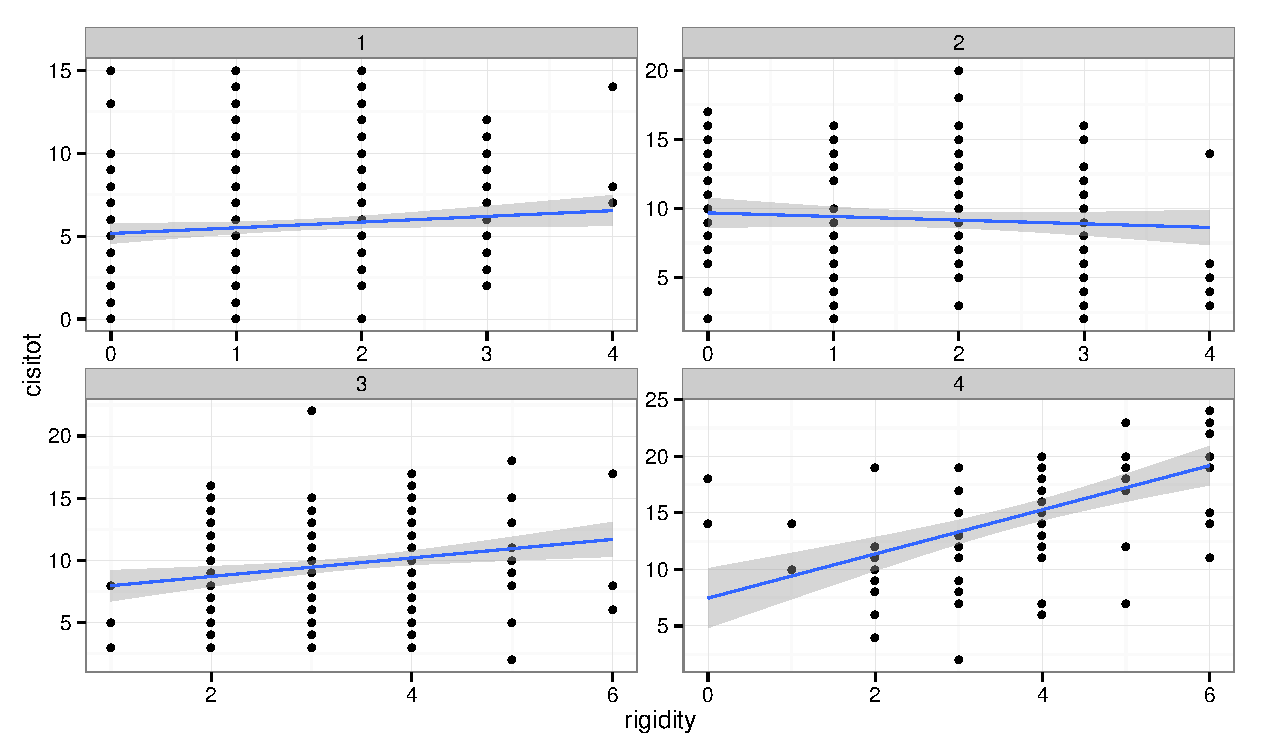
\includegraphics[clip,width=\linewidth]{rigidity-v-cisitot.pdf}
  \label{rigidv}
}
  \caption{Relationship between \protect\subref{bradyv} bradykinesia,
  \protect\subref{rigidv} rigidity and overall severity (cisitot). Shaded band
is 95\% confidence interval.}
  \label{fig:corrxy-br}
\end{figure}

\begin{figure}[H]
  \centering
  \subfloat[][]{%
  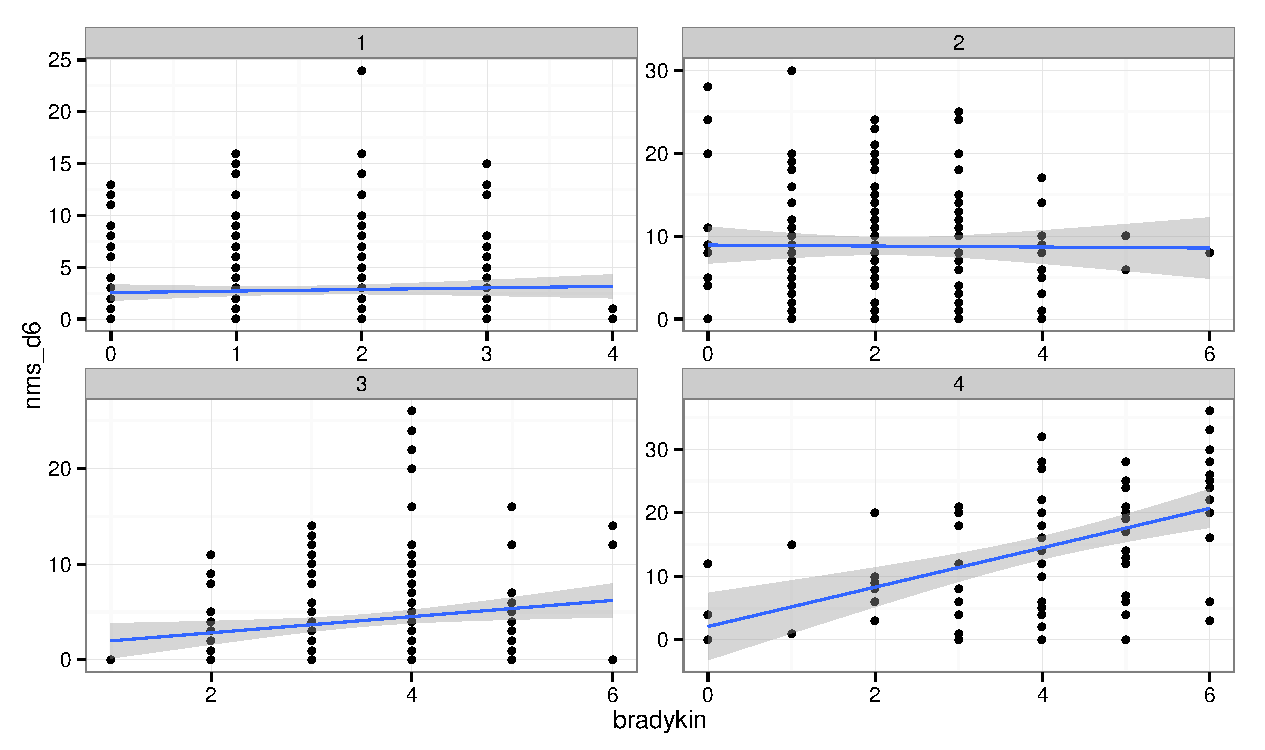
\includegraphics[clip,width=\linewidth]{bradykin-v-nms_d6.pdf}
  \label{brady6}
}

\subfloat[][]{%
  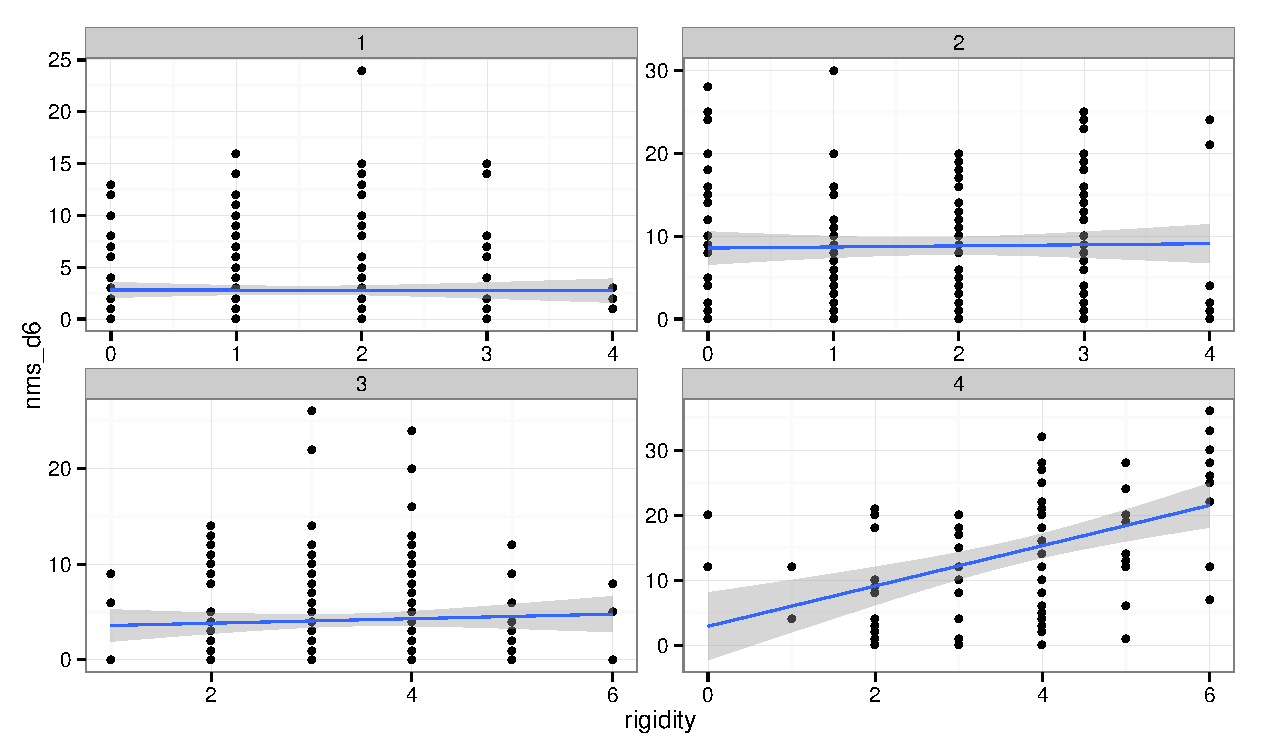
\includegraphics[clip,width=\linewidth]{rigidity-v-nms_d6.pdf}
  \label{rigid6}
}
  \caption{Relationship between \protect\subref{brady6} bradykinesia,
  \protect\subref{rigid6} rigidity and nms\_d6 (gastrointestinal). Shaded band
is 95\% confidence interval.}
  \label{fig:corrxy-d6}
\end{figure}
\begin{figure}[H]
  \centering
  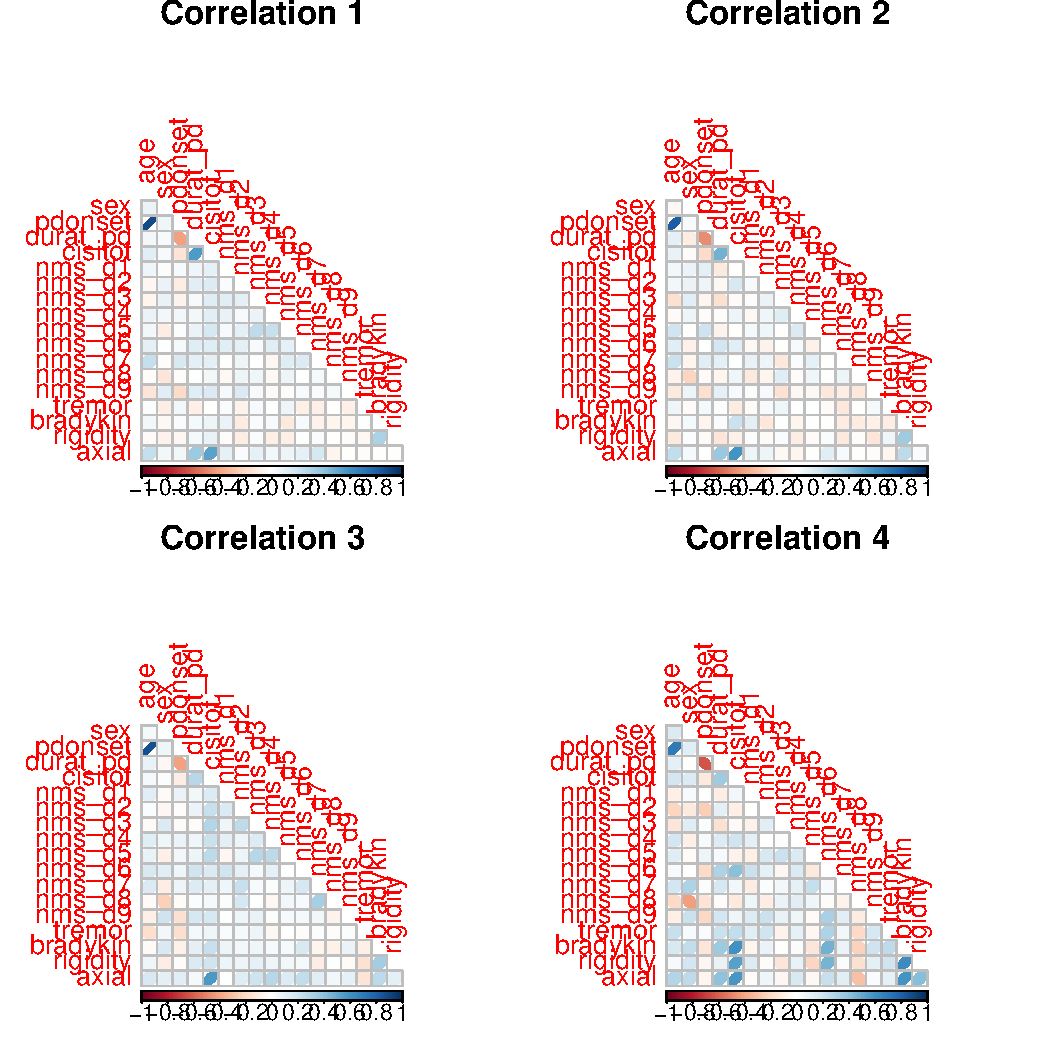
\includegraphics[width=\linewidth]{corrplots.pdf}
  \caption{Correlation plots}
  \label{fig:corrplots}
\end{figure}

\section{Nonmotor-predominant subtype analysis}
\subsection{$k$-means sub-subdivision on Cluster 2}
% TODO: Synthesize changed subtype 2 analysis with discussion HERE and in
% conclusion. Make sure to reread and ensure that all plots have been updated
% (in particular, the 4 cluster decision tree?). Incorporate some stuff from
% standard progression of motor diseases paper and the new nms subtype paper.

In an attempt to understand further the properties of the nonmotor-dominated
subtypes, $k$-means analysis was run again on specifically this subtype to
examine any possible patterns.

The same $k$-determining tests were run on subtype 2 and are displayed
in Table~\ref{tab:numclus-nms}.

\begin{table}[H]
  \centering
  \begin{tabular}{l|l}
    Criterion & Optimal $k$ \\
    \hline
    Minimum ASW & 2 \\
    BIC & 1 (?) \\
    SSE Scree Plot & Inconclusive \\
    Gap Statistic & 3 \\
    Affinity Propagation\tablefootnote{$\lambda = 0.98$, q = 0, maxits = 1000,
    convits = 100} & 5 \\
  \end{tabular}
  \caption{Results of various techniques for determining $k$, applied to
  subtype 2}
  \label{tab:numclus-nms}
\end{table}

Boxplots for $k$-means run for $k = 2, 3, 4$ can
be seen in Figures~\ref{fig:c2-summaries-2},~\ref{fig:c2-summaries-3},
and~\ref{fig:c2-summaries-4}. Clusters are ordered by increasing cisitot.

\subsection{Interpretation}
\label{sub:nms-interp}

An interesting set of subtleties occurs when $k = 2$ and 3. When $k = 2$, the
two groups are divided generally by PD severity (see cisitot and especially
axial). The specific symptoms of the two groups follow this trend, except
nms\_d3 and tremor, which are actually decreasing, and other symptoms like
rigidity, nms\_d4, and nms\_d9, which are more indeterminate.

When $k = 3$, the symptoms that continue show a non-monotonically increasing
trend are nms\_d2, tremor, and rigidity scores, where patients in the 3rd
subtype exhibit lower severities. nms\_d4 and nms\_d9 differences turn out to be
not as pronounced.

\begin{figure*}[p]
  \centering
  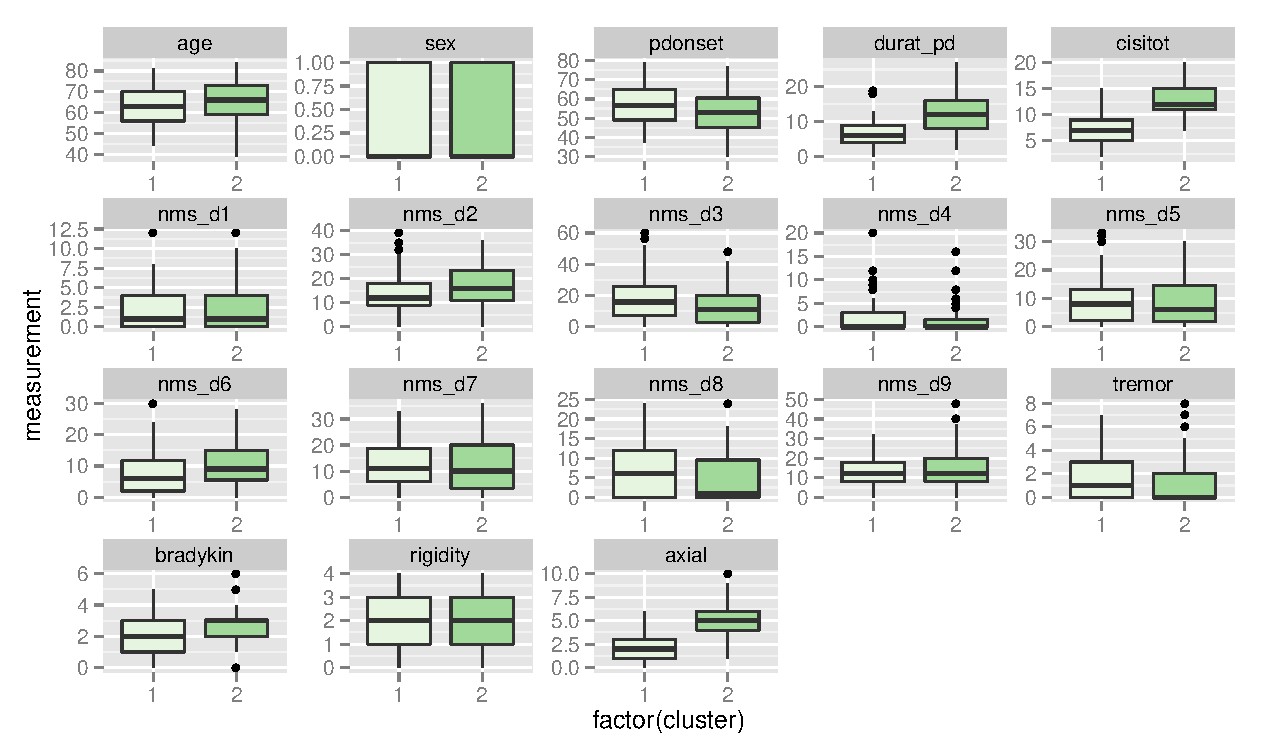
\includegraphics[width=0.65\linewidth]{c2-summaries-2.pdf}
  \caption{Clustering on nonmotor group: $k = 2$}
  \label{fig:c2-summaries-2}
\end{figure*}
\begin{figure*}[p]
  \centering
  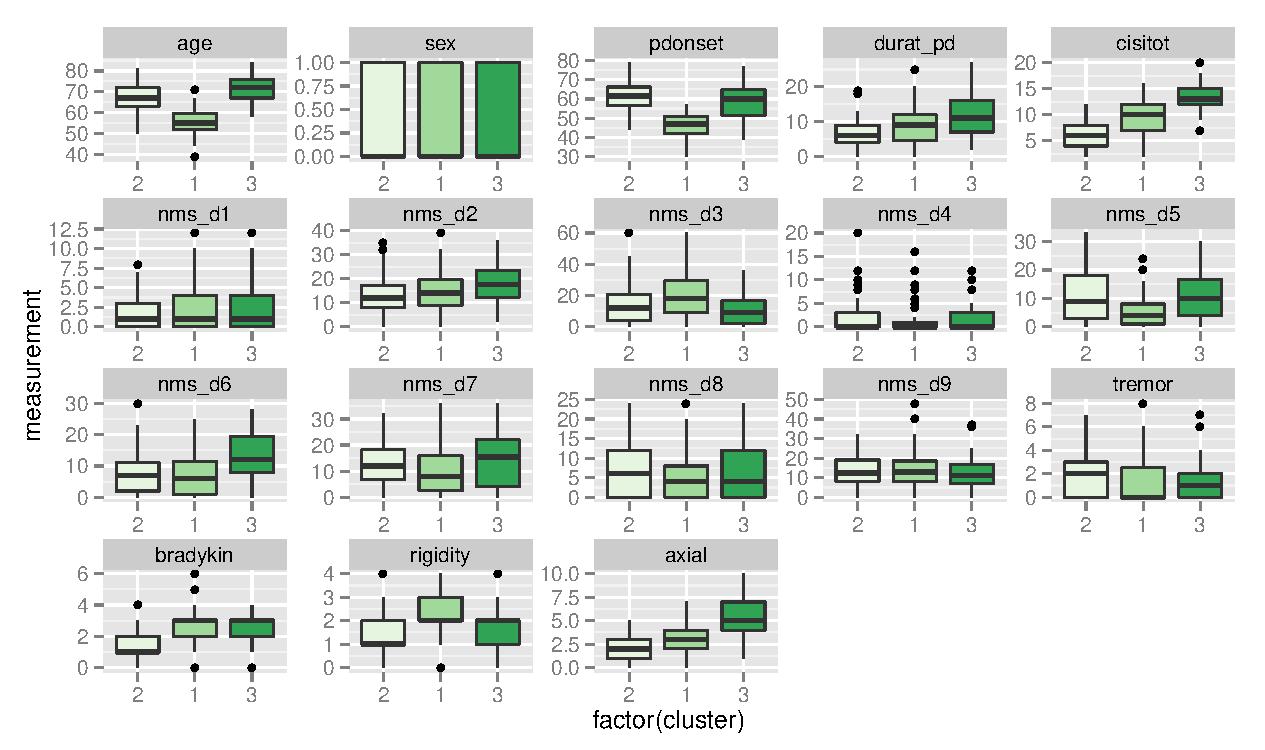
\includegraphics[width=0.65\linewidth]{c2-summaries-3.pdf}
  \caption{Clustering on nonmotor group: $k = 3$}
  \label{fig:c2-summaries-3}
\end{figure*}
\begin{figure*}[p]
  \centering
  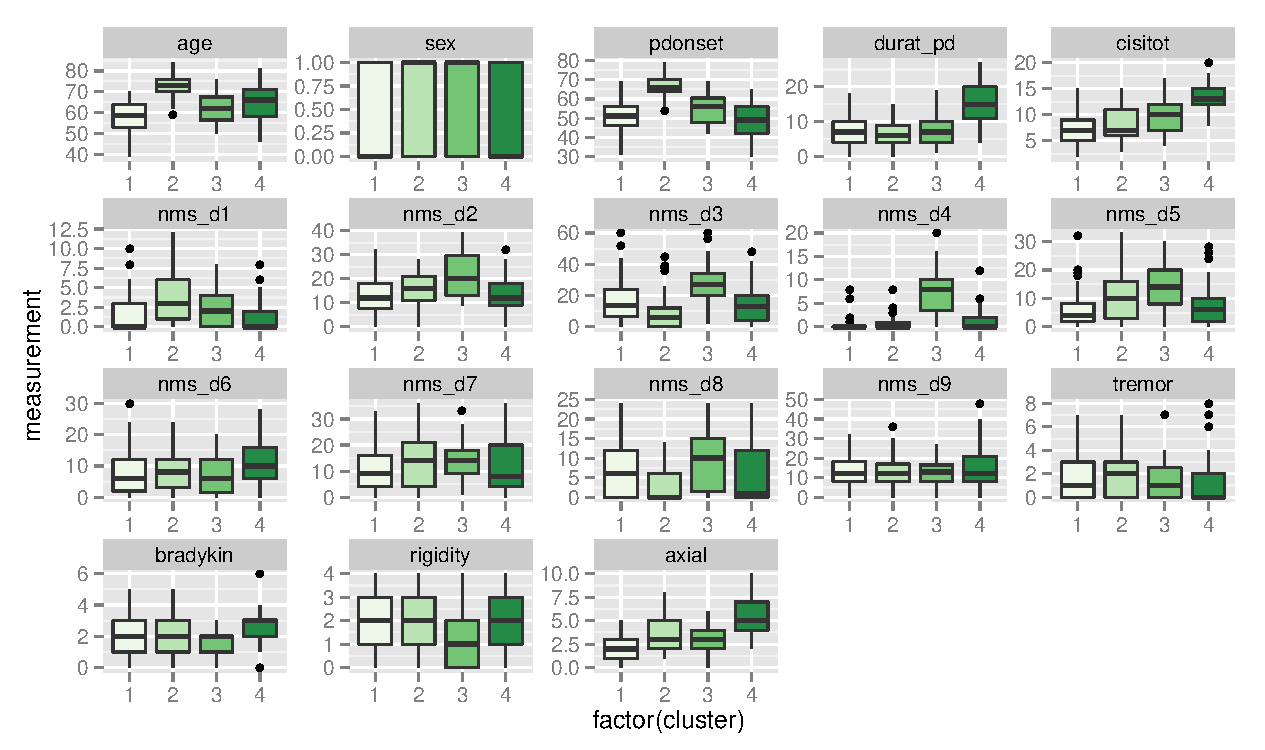
\includegraphics[width=0.65\linewidth]{c2-summaries-4.pdf}
  \caption{Clustering on nonmotor group: $k = 4$}
  \label{fig:c2-summaries-4}
\end{figure*}


\section{Further modeling}

One further step of this investigation was to produce accurate, practical
models that could be used in a clinical setting to predict the subtype of PD
based on previous clustering results. Cluster assignments obtained from
previous $k$-means investigation were treated as labels in a supervised
classification problem in an attempt to produce useful and easily interpretable
models.

\subsection{One-versus-all decision trees}
\label{sub:ova}

While the decision tree in Figure~\ref{fig:kmeans-dtree-4} is useful, it could
be considered overly complicated. Additionally, a model is not necessarily
needed to make simpler diagnoses such as classifying a patient as mildly
affected (subtype 1) or severely affected (subtype 4). One-versus-all (OVA)
decision trees were thus considered, in order to isolate the classification
problem and look at possible distinguishing characteristics of individual
subtypes. These OVA decision trees for all 4 subtypes are located in
Figures~\ref{fig:1va},~\ref{fig:2va},~\ref{fig:3va}, and~\ref{fig:4va}. Trees
are pruned by selecting the version of tree with the minimum 10-fold
cross-validated error.

\subsubsection{1 (mild)}
The tree for the mild subtype classifies mainly based on negative responses to
nodes asking whether the patient has a relatively severe manifestation of a
symptom. The majority of examples are classified by following the bradykinesia
$<$ 2.5, which subsequently tests the severity of several nonmotor symptoms.
Most of subtype 1 patients that score relatively mildly on these scales are
classified this way. There are also small populations of patients who 1) score
% http://www.ncbi.nlm.nih.gov/pubmed/22233888
higher on bradykinesia but lower with axial, tremor, rigidity, and nms\_d2 and
2) score higher in nms\_d2 (sleep) but lower with nms\_d7 (urinary).
% This tree is very odd. The root node considers nms\_d9 $< 7.5$  and nms\_d3 (miscellaneous)
% and classifies by far the biggest majority of negative examples when this
% symptom is milder, even though the subgroup 1 is the mild subtype. After
% intuitively then classifying on the mildness of rigidity (rigidity >= 3.5) the tree then proceeds
% to classify once again negative examples mostly based on mildness of nms\_d2
% (sleep)
% and positive examples based on more severe manifestations of nms\_d2,
% despite the means of these nonmotor symptoms being quite similar according to
% the boxplots.  However, accuracy on the final nodes are quite poor, which could
% be an indicator that the cluster is not well defined.

\subsubsection{2 (nonmotor-predominant)}
The decision tree for the nonmotor-predominant subtype is quite simple.
Interestingly, although nms\_d9 (miscellaneous) is not the most important
nonmotor symptom, since the information gain is less than nms\_d2 and nms\_d3
and it does not appear very high in the 4-class decision tree, it is used as
the root node of this decision tree, classifying over half of the negative
examples based on whether the subject has a low severity of miscellaneous
symptoms (nms\_d9 $<$ 7.5)\footnote{Recall that 0 $<$ nms\_d9 $<$ 48.}. This could be an indication that nonmotor-predominant PD patients do
indeed have a wide manifestation and variety of nonmotor symptoms. After
classifying on nms\_d9, the tree then classifies negatiave examples as having
rigidity $\geq$ 3.5, an example of how subtype 2 patients have relatively low motor
symptoms. Finally, the tree classifies on the nonmotor symptom with the most
information gain, nms\_d2, where patients $\geq$ 7.5 are classified as falling into
subtype 2.

% Quite characteristically, this OVA decision tree clusters first on the severity
% of bradykinesia. When mild (i.e.\ bradykin $< 2.5$), all of the subsequent decision
% nodes ask whether the patient has correspondingly severe forms of primarily
% nms\_d3 (mood/cognition), then nms\_d7 (urinary) and nms\_d9 (miscellaneous).

% When bradykinesia (and all motor symptoms) are relatively severe, however,
% there is still a small subset of patients who classify into subtype 2 by having
% severe nms\_d2 (sleep) symptoms. While I am not sure if the sample size is
% large enough here (9/34), I propose this could be one of the ``subtypes'' of
% the nonmotor-predominant subtype, i.e.\ a group that, when accompanied with
% high motor symptoms, generally will have high nonmotor symptoms manifest
% primarily in the form of sleep disorders. This aligns with the findings
% previously mentioned in Section~\ref{sub:nms-interp} a disjunct between
% symptoms nms\_d2 and nms\_d3. As briefly mentioned in that section, axial motor
% symptom severity also plays a role. In this tree, mildness of axial symptoms is
% the main classifier of 280 negative examples when identifying
% nonmotor-predominant
% subtypes, indicating it is an important distinguishing factor of this unique
% group of 34 nonmotor-predominant PD patients.

% More discussion on this decision tree, synthesized with the other results of
% this research, is in the conclusion.

\subsubsection{3 (motor-predominant)}

This tree classifies overwhelmingly on severity of bradykinesia, with 476
negative examples when bradykinesia is less than 2.5. The resulting tree is
quite complex, but generally, nodes check again for severity of motor
symptoms (tremor is the next node) and end up classifying positive examples
based on both mildness of nonmotor symptoms and severity of motor symptoms. For
example, in the furthest right branch, once nms\_d2 (as we know, an important
feature) is established to be relatively mild ($<$ 12), the test for subtype 3
involves several more nodes verifying the severity of rigidty, tremor, and
axial, and the mildness of nms\_d7 (urinary).

\subsubsection{4 (severe)}

The OVA tree for patients severely affected in all areas is predictable, testing
entirely on whether or not symptoms (both motor and nonmotor) are relatively
severe. Positive nodes always appear to the right (no) of less-than checks.
Interestingly, however, nms\_d4 (percep/hallucinations), previously not of note, is used twice as the
root node of a tree and again further down. As the boxplot display in
Figure~\ref{fig:kmeans-summaries-4} shows, nms\_d4 is perhaps the most
distinguishing symptom of subtype 4 against nonmotor-predominant
subtype 2 in particular, as subtype 2 has relatively mild percep/hallucination
symptoms, in contrast to the comparable levels of severity for other nonmotor
symptoms in both groups. This shows that issues with perception and
hallucinations generally occur in only the most severe cases of PD, and are
relatively rare when a patient exhibits a nonmotor-predominant form of PD.

\begin{figure}[H]
  \centering
  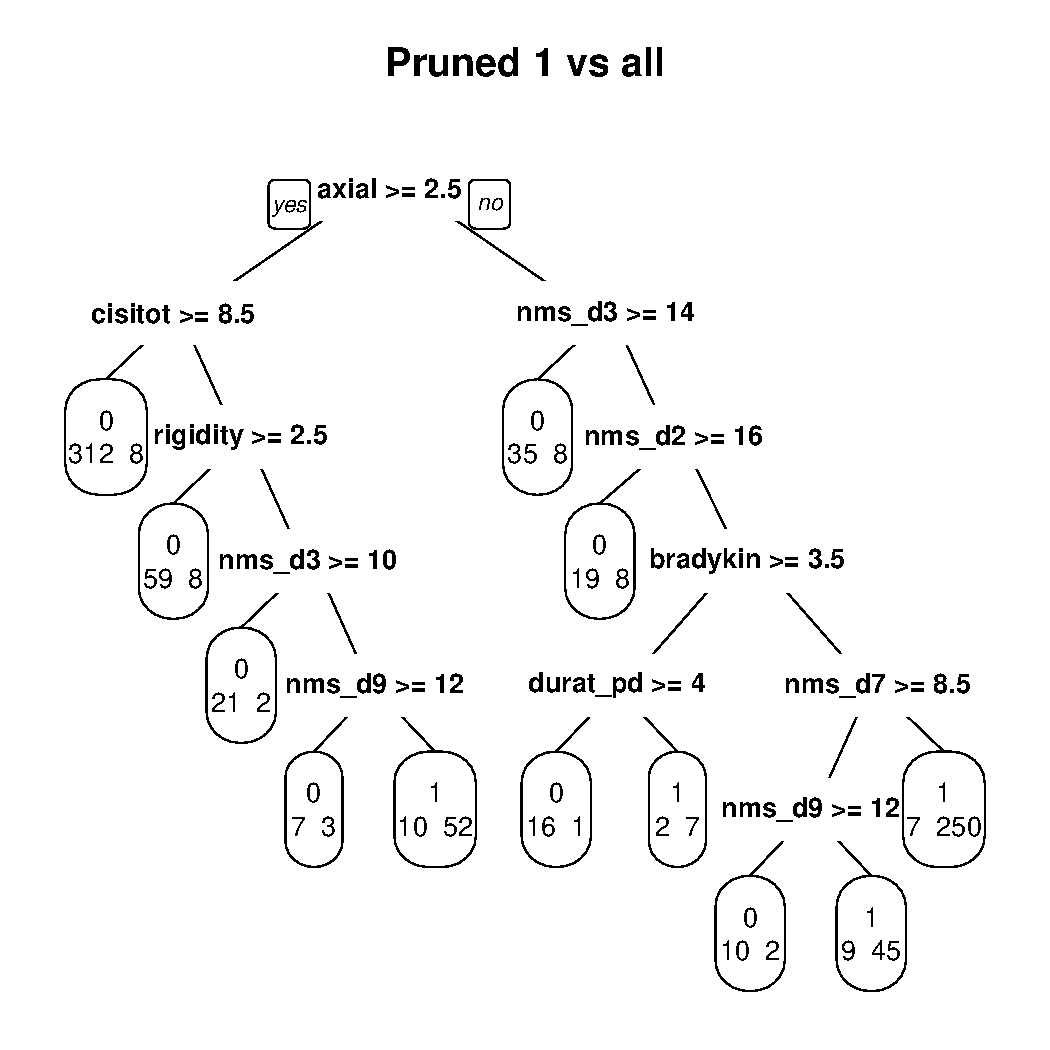
\includegraphics[width=0.75\linewidth]{dtree-1va-pruned.pdf}
  \caption{Cluster 1 (mild) vs all}
  \label{fig:1va}
\end{figure}

\begin{figure}[H]
  \centering
  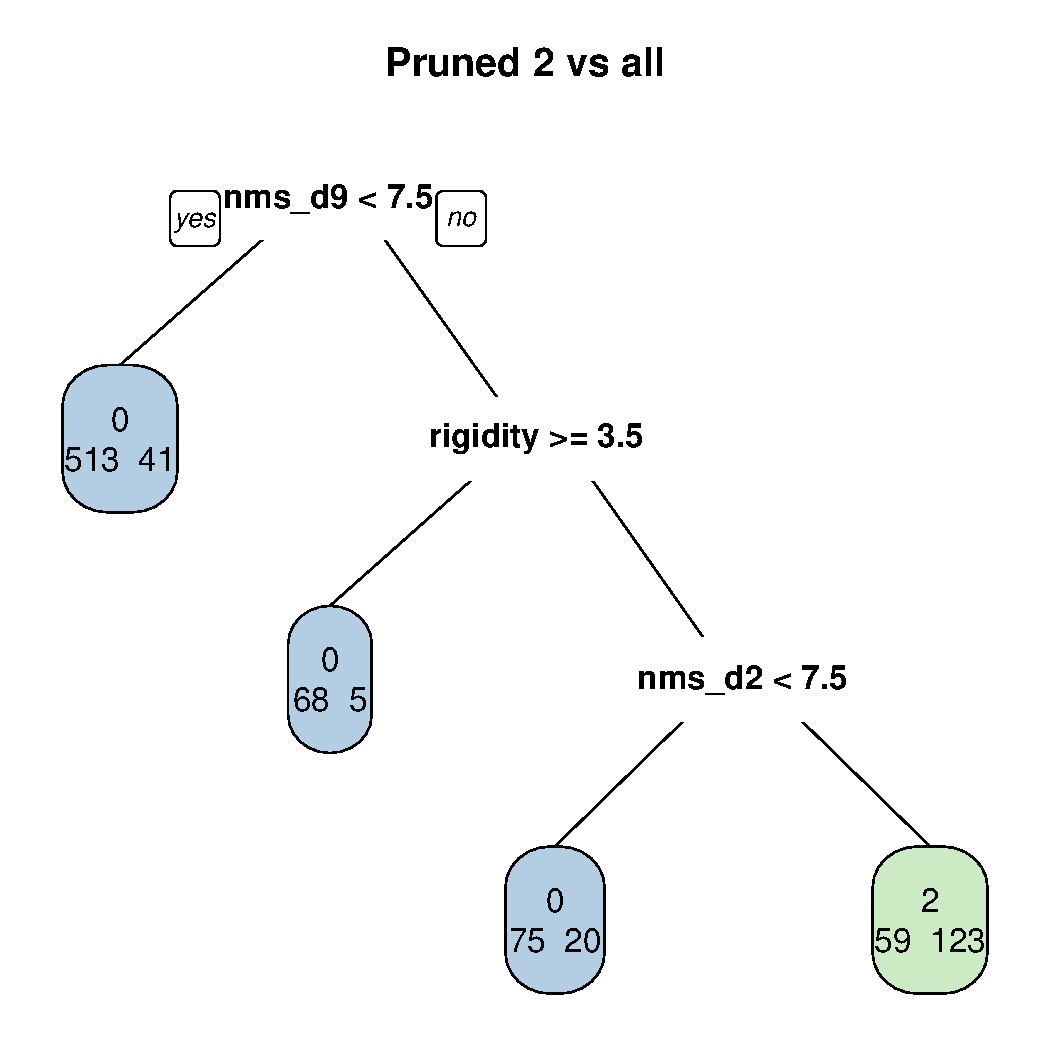
\includegraphics[width=0.75\linewidth]{dtree-2va-pruned.pdf}
  \caption{Cluster 2 (nonmotor-dominated) vs all}
  \label{fig:2va}
\end{figure}
\begin{figure}[H]
  \centering
  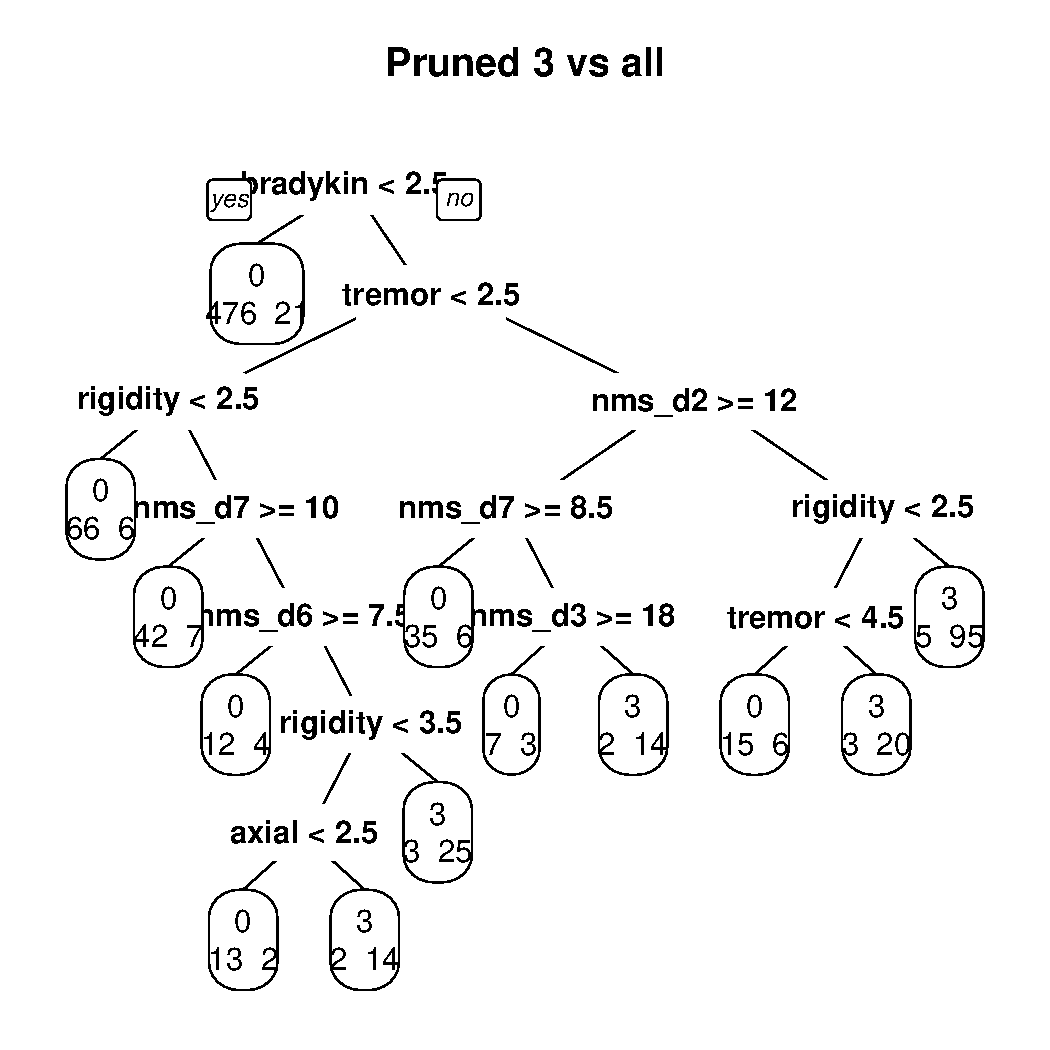
\includegraphics[width=0.75\linewidth]{dtree-3va-pruned.pdf}
  \caption{Cluster 3 (motor-dominated) vs all}
  \label{fig:3va}
\end{figure}
\begin{figure}[H]
  \centering
  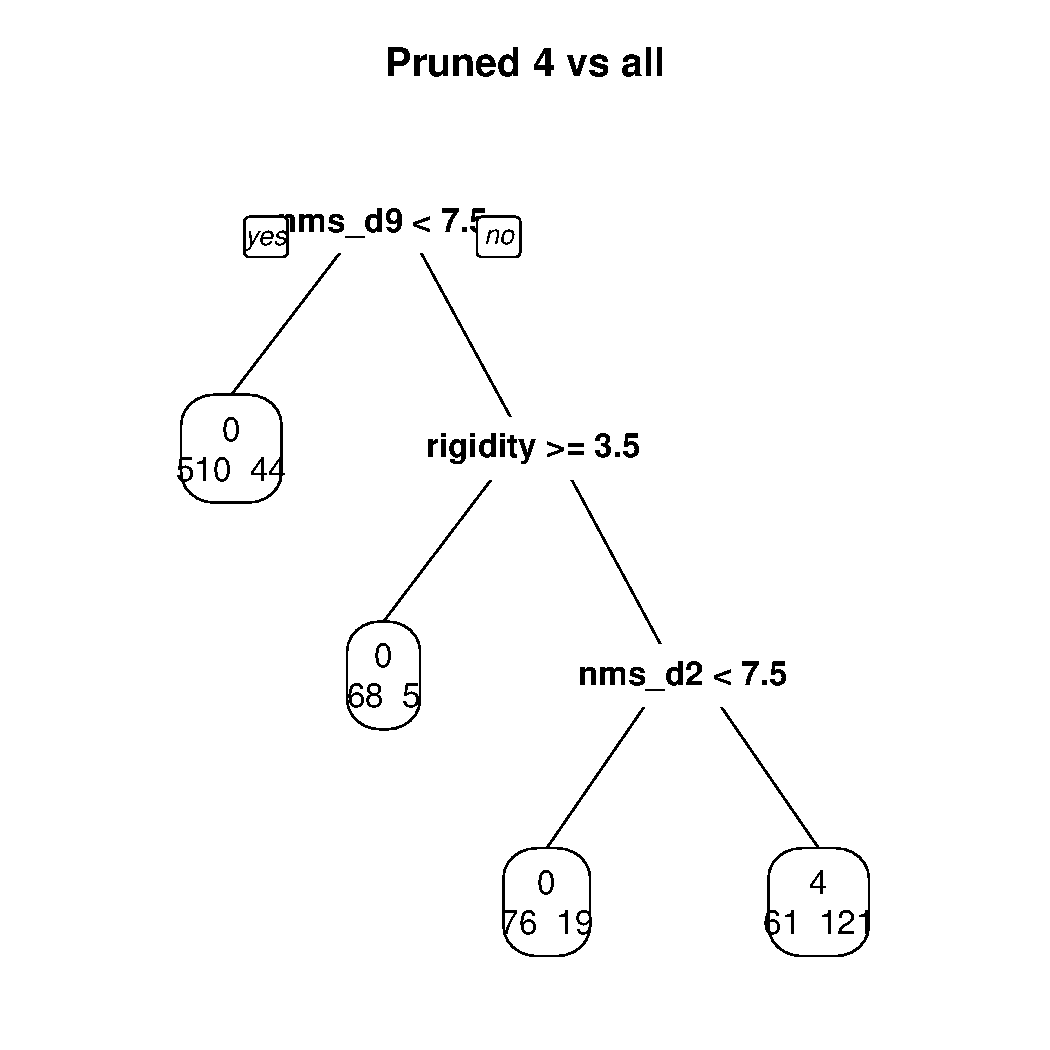
\includegraphics[width=0.75\linewidth]{dtree-4va-pruned.pdf}
  \caption{Cluster 4 (severe) vs all}
  \label{fig:4va}
\end{figure}

\subsection{Different angles of exploration: 2 and 4, 2 and 3 vs rest}

There are many more interesting questions to be asked when examining the
relationship between these clusters. One thing that may be helpful in
understanding the relationship between the clusters is exploring different
groupings of clusters for decision trees. The trees in
Figure~\ref{fig:dtree-2and4va-pruned} and~\ref{fig:dtree-2and3va-pruned} are
preliminary examples of this kind
of exploration.

\subsubsection{2 and 4 vs rest}
In this tree, the node classifying examples as subtype 4 is
localized to the furthest right branch. Predictably, examples in this node have
scored relatively higher in rigidity ($\geq$ 3.5). Interestingly, a classification
decision that is replicated in the 4 versus all decision tree is the decision
to use nms\_d7 (urinary) as a node, where subtype 4 is classified as having
relatively high nms\_d7 components ($\geq$ 12). Indeed, as shown in
Figure~\ref{fig:kmeans-summaries-4}, the mean of nms\_d7 severity is similar to
nms\_d4 in that it is especially higher in cluster 4 than in cluster 2.

\subsubsection{2 and 3 vs rest}
In this tree, classification of patients in subtype 3 is primarily dependent on
asserting bradykin $\geq$ 2.5 then splitting on tremor $<$ 3.5 is considered.
Interestingly, the two nonmotor symptoms that differentiate cluster 3 are
nms\_d5 (attention/memory) and nms\_d7 (urinary). Additionally, nms\_d2, a
quite important symptom, does not appear in the classification tree for this
task.

\begin{figure}[H]
  \centering
  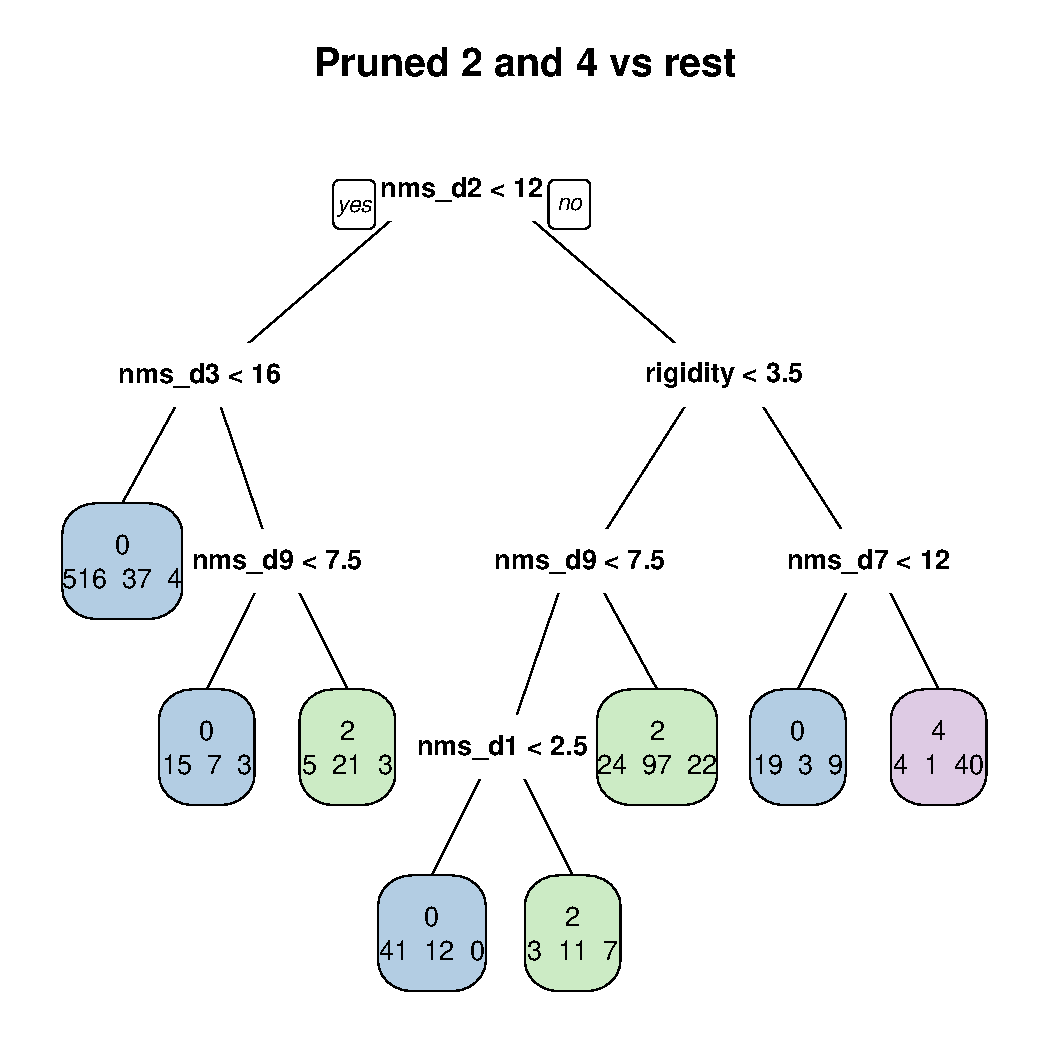
\includegraphics[width=0.75\linewidth]{dtree-2and4va-pruned.pdf}
  \caption{Clusters 2 (nms) and 4 (severe) vs rest (1 and 3)}
  \label{fig:dtree-2and4va-pruned}
\end{figure}

\begin{figure}[H]
  \centering
  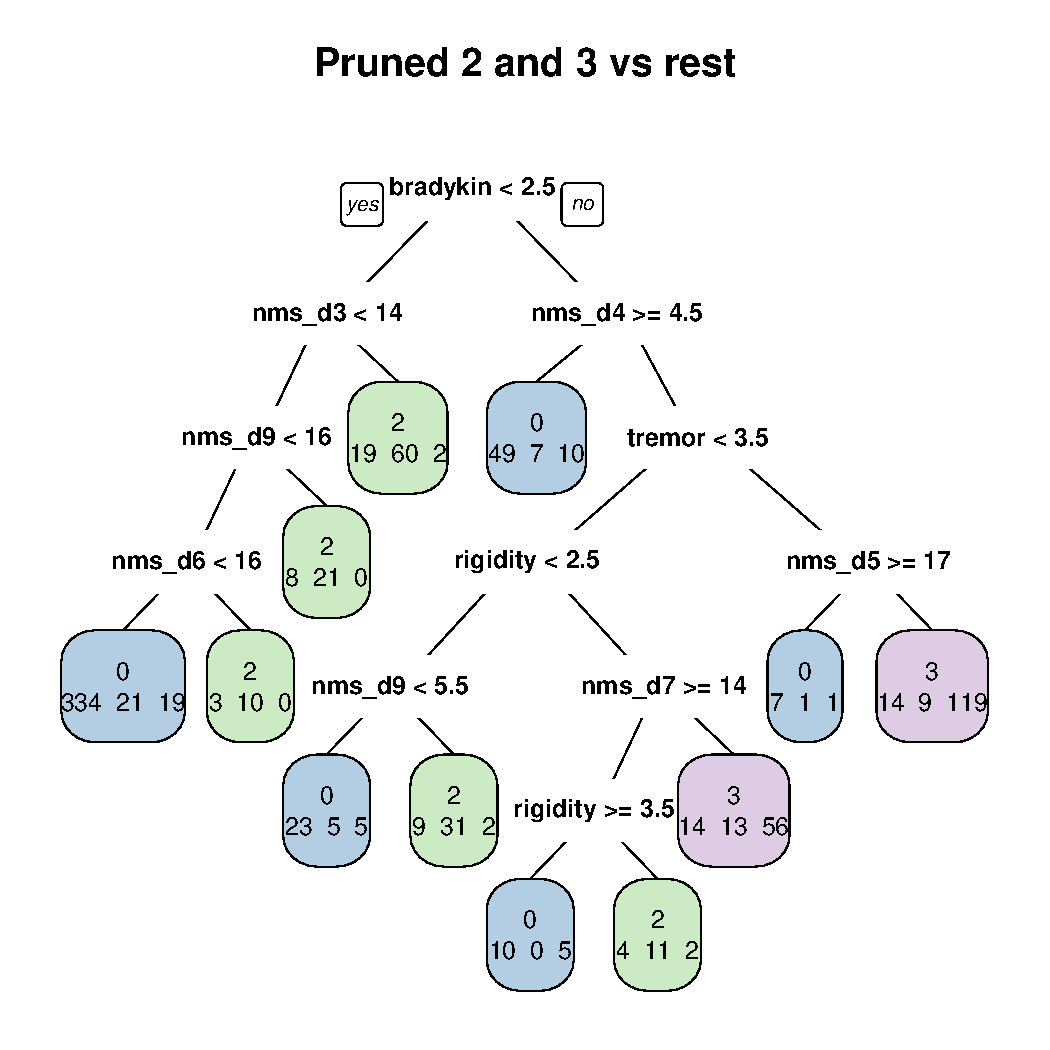
\includegraphics[width=0.75\linewidth]{dtree-2and3va-pruned.pdf}
  \caption{Clusters 2 (nms) and 3 (motor) vs rest (1 and 4)}
  \label{fig:dtree-2and3va-pruned}
\end{figure}

\subsection{Bayesian Networks}

\subsubsection{On all data}

I decided to discretize the data into three uniform-width groups based on the
scales of each symptom. In other words, each symptom was discretized into a
mild, moderate, and severe bin. Continuous data was unreliable on my computer,
and updating intricately connected nodes like nms\_d2 resulted in slowdowns and
crashes on my computer.

Two bayesian network algorithms were tried: the default Bayesian score-search
algorithm and the PC conditional independence tests algorithm. I couldn't find
the exact name of the Bayesian search implementation, but it was the default
method used by GeNIe. GeNIe files will be attached electronically.

I assume these models are to be looked at by Dr. Mart\'in. I have not done too
much investigation myself, as I'm not exactly sure what I'm looking for.

\subsubsection{On nms-dominated data}
I tried to construct Bayesian networks based on the nms-dominated subtype, but
the data was too sparse to create a very informative network, even when leaving
the information continuous. However, I'm not sure this is necessary. If it is,
I can work on this problem more.



\section{Longitudinal Analysis}
\label{sec:longitudinal}

I wanted to observe the progression of nonmotor symptoms of Parkinson's disease akin to work done
by various studies (e.g.\ \cite{onsetpd,vu12,zahodne12}). The data was a little bit too noisy when
I tried to examine correlations, so I decided to average the values into bins for
\texttt{durat\_pd}: 0-2 years, 2-4 years, 4-6 years, etc. First, the correlation based on PD
duration for each symptom is displayed in Figure~\ref{fig:longcorr}.

\begin{quote}
  Note: I have not included all of the graphs I have, just those I found interesting. If you would
  like all of the graphs, I can send those to you in a separate email.
\end{quote}


\begin{figure*}[t]
  \centering
  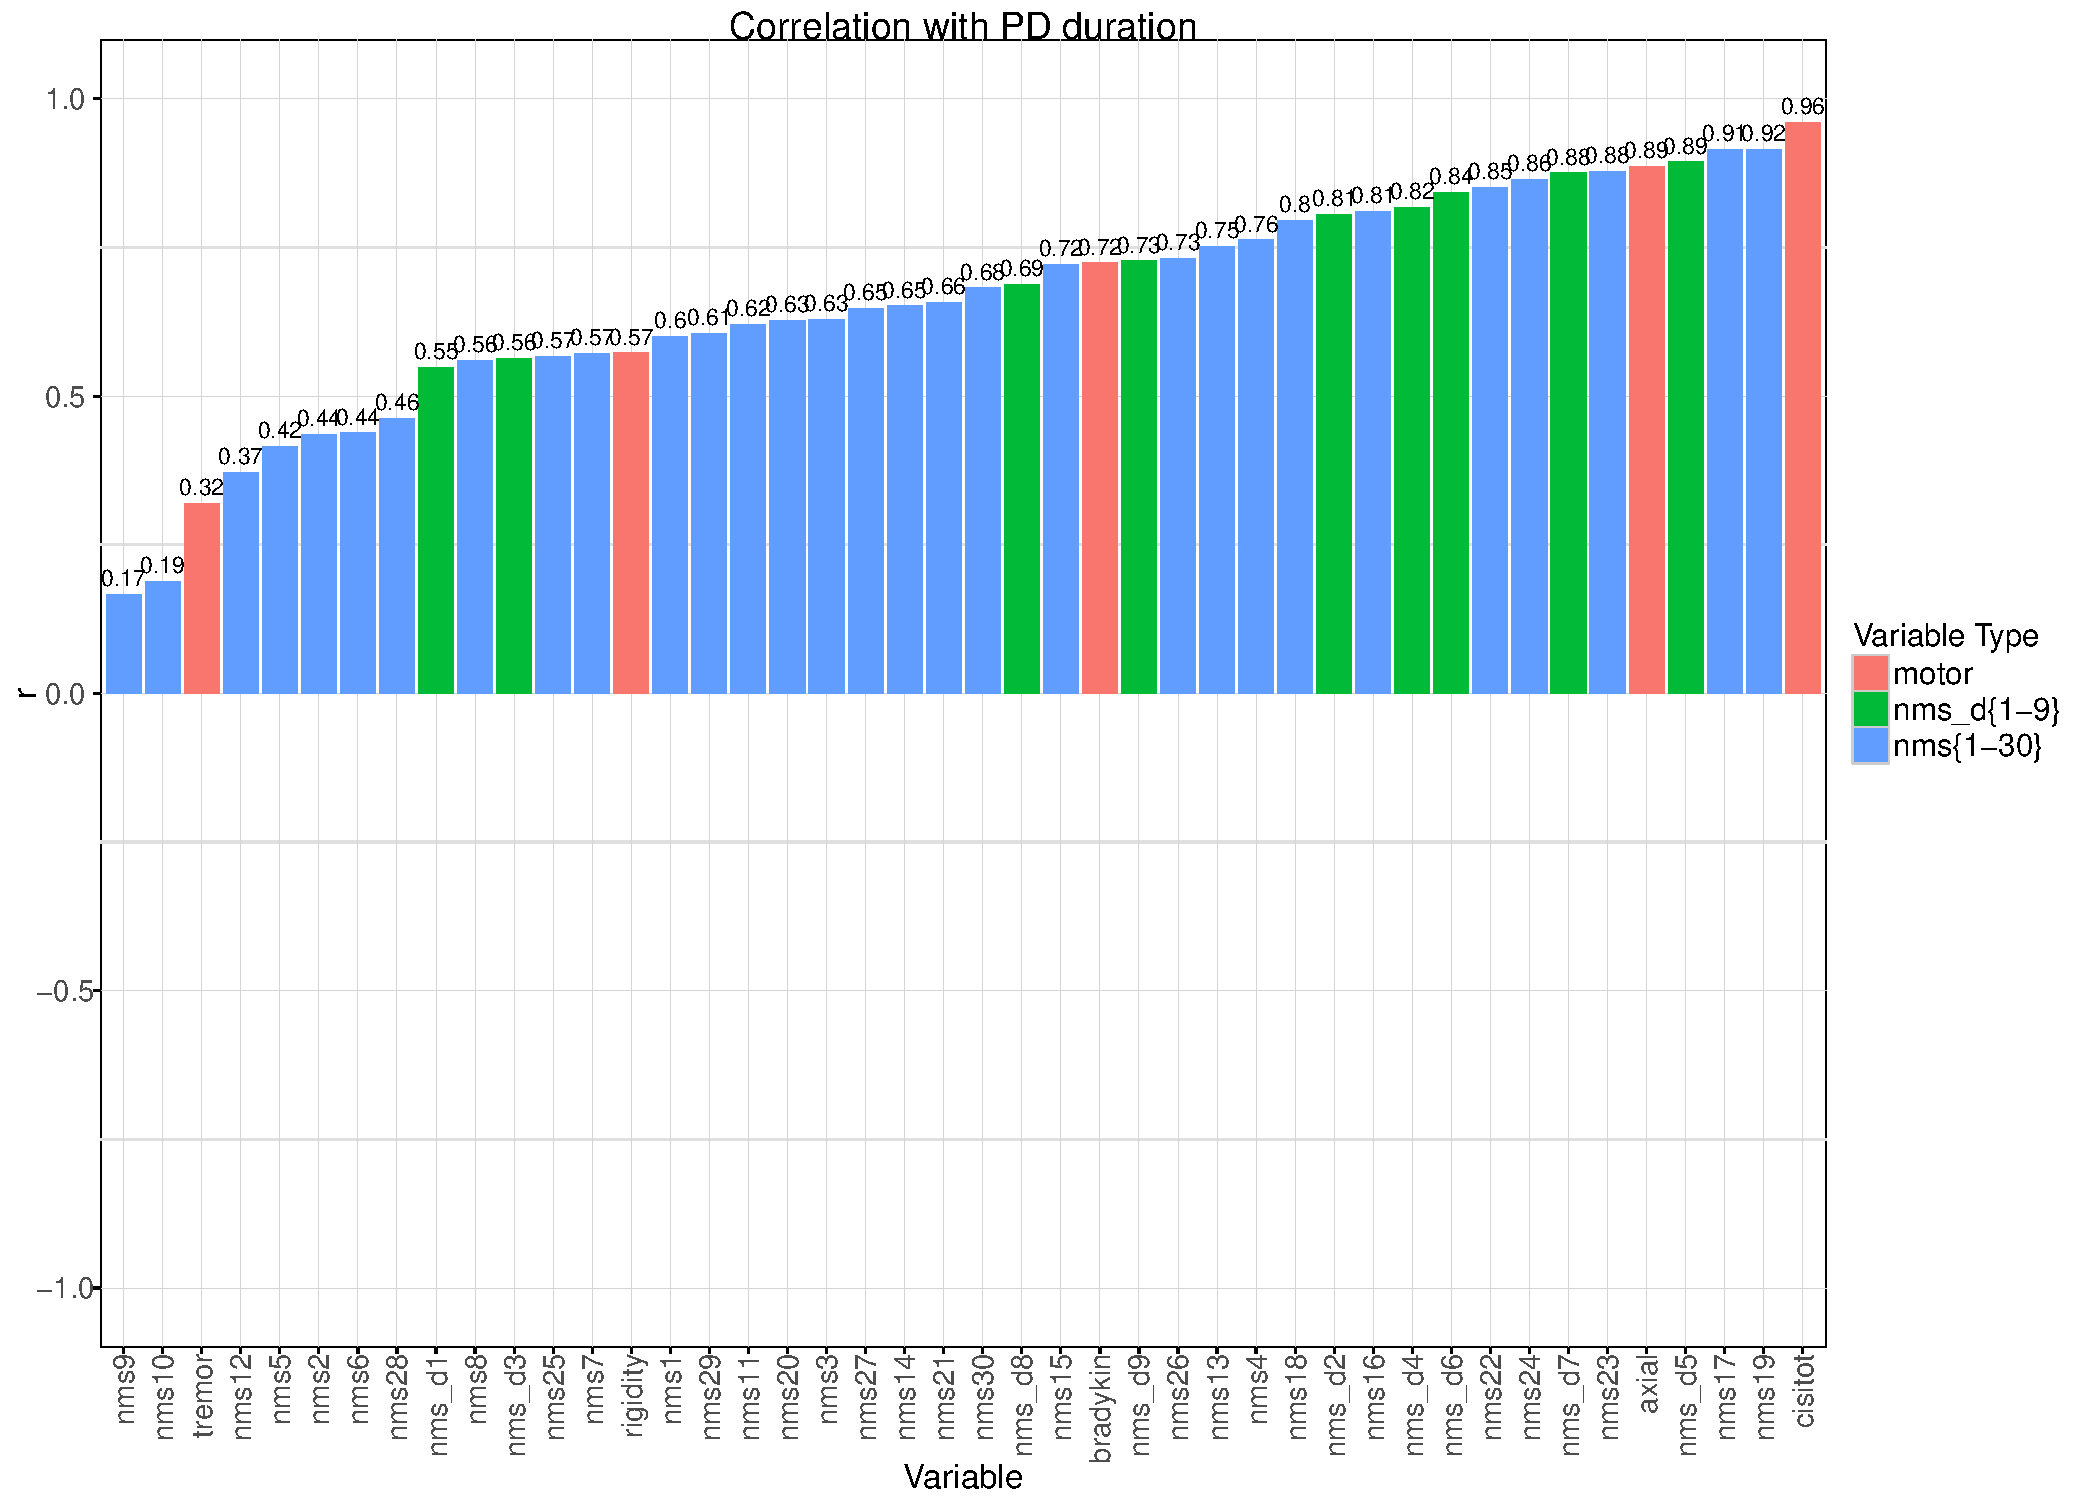
\includegraphics[width=0.9\linewidth]{pd-durat-cor.pdf}
  \caption{Correlation of variables according to PD Duration}
  \label{fig:longcorr}
\end{figure*}

Most symptoms have at least a minor positive correlation. Interestingly, tremor, nms9 (anxiety)
and nms10 (depression) do not have a strong correlation with PD duration.
% This could give evidence that whether or not someone has high tremor is a distinct subtype?

\subsection{Anxiety}
I plotted the mean nms\_9 (anxiety) score for each durat\_pd bin in
Figures~\ref{fig:nms9-long} and ~\ref{fig:nms9-multi}

\begin{figure*}[p]
  \centering
  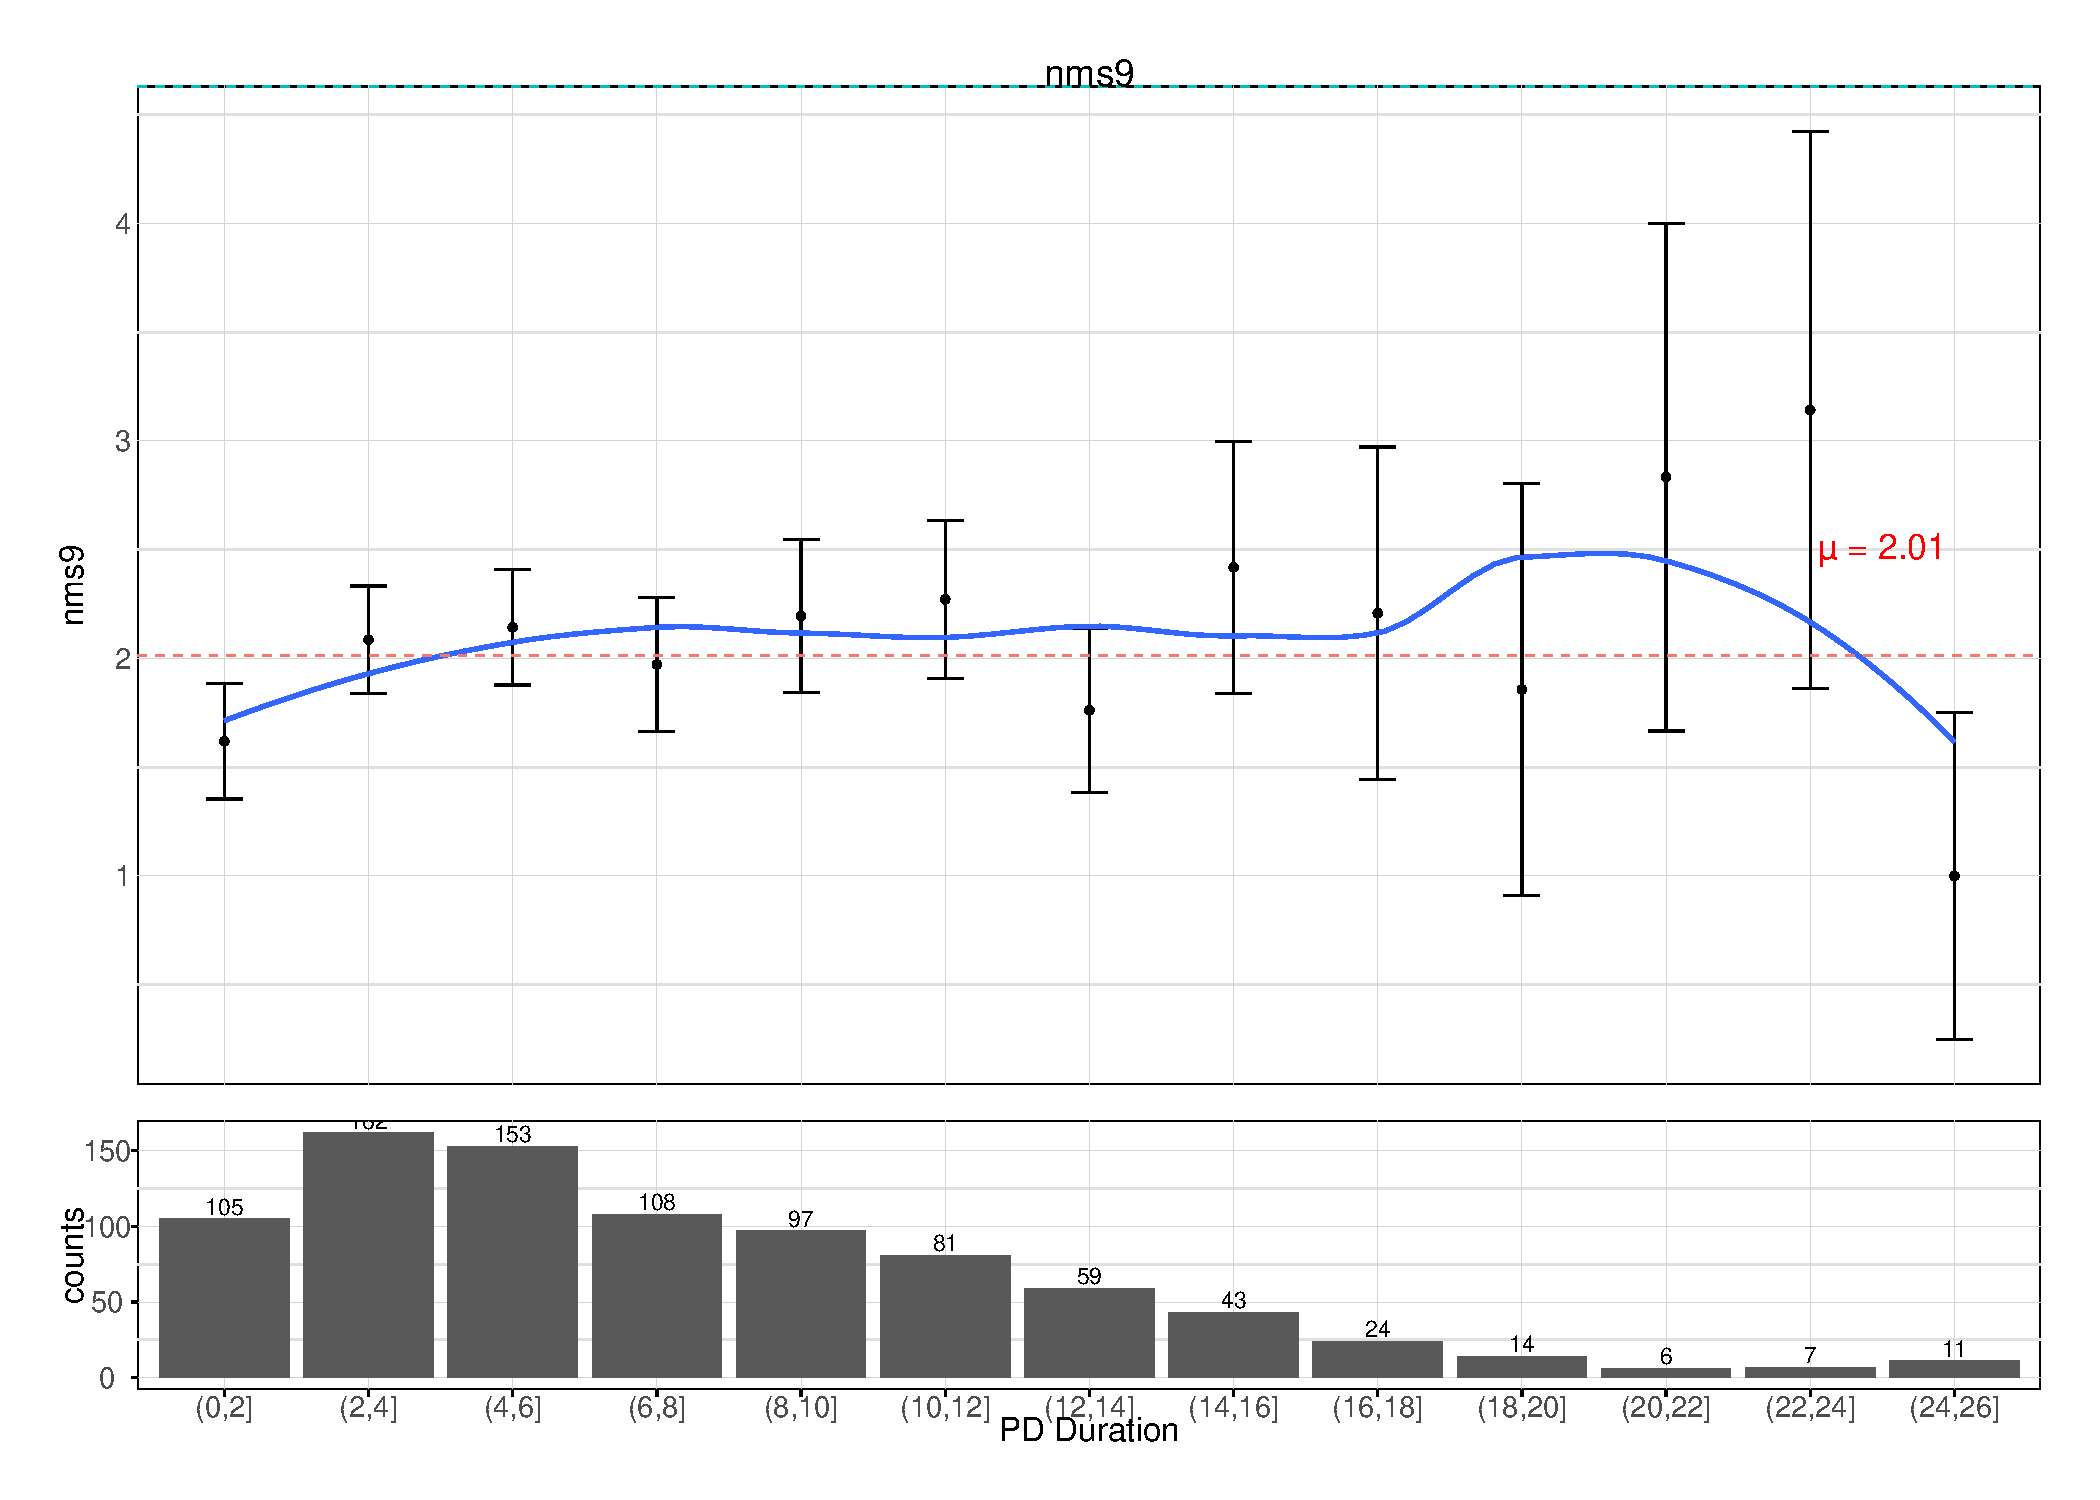
\includegraphics[width=0.8\linewidth]{nms9-durat-counts.pdf}
  \caption{Mean anxiety (nms\_9) score by PD duration, with number of patients in each group at
  bottom.}
  \label{fig:nms9-long}
\end{figure*}

\begin{figure*}[p]
  \centering
  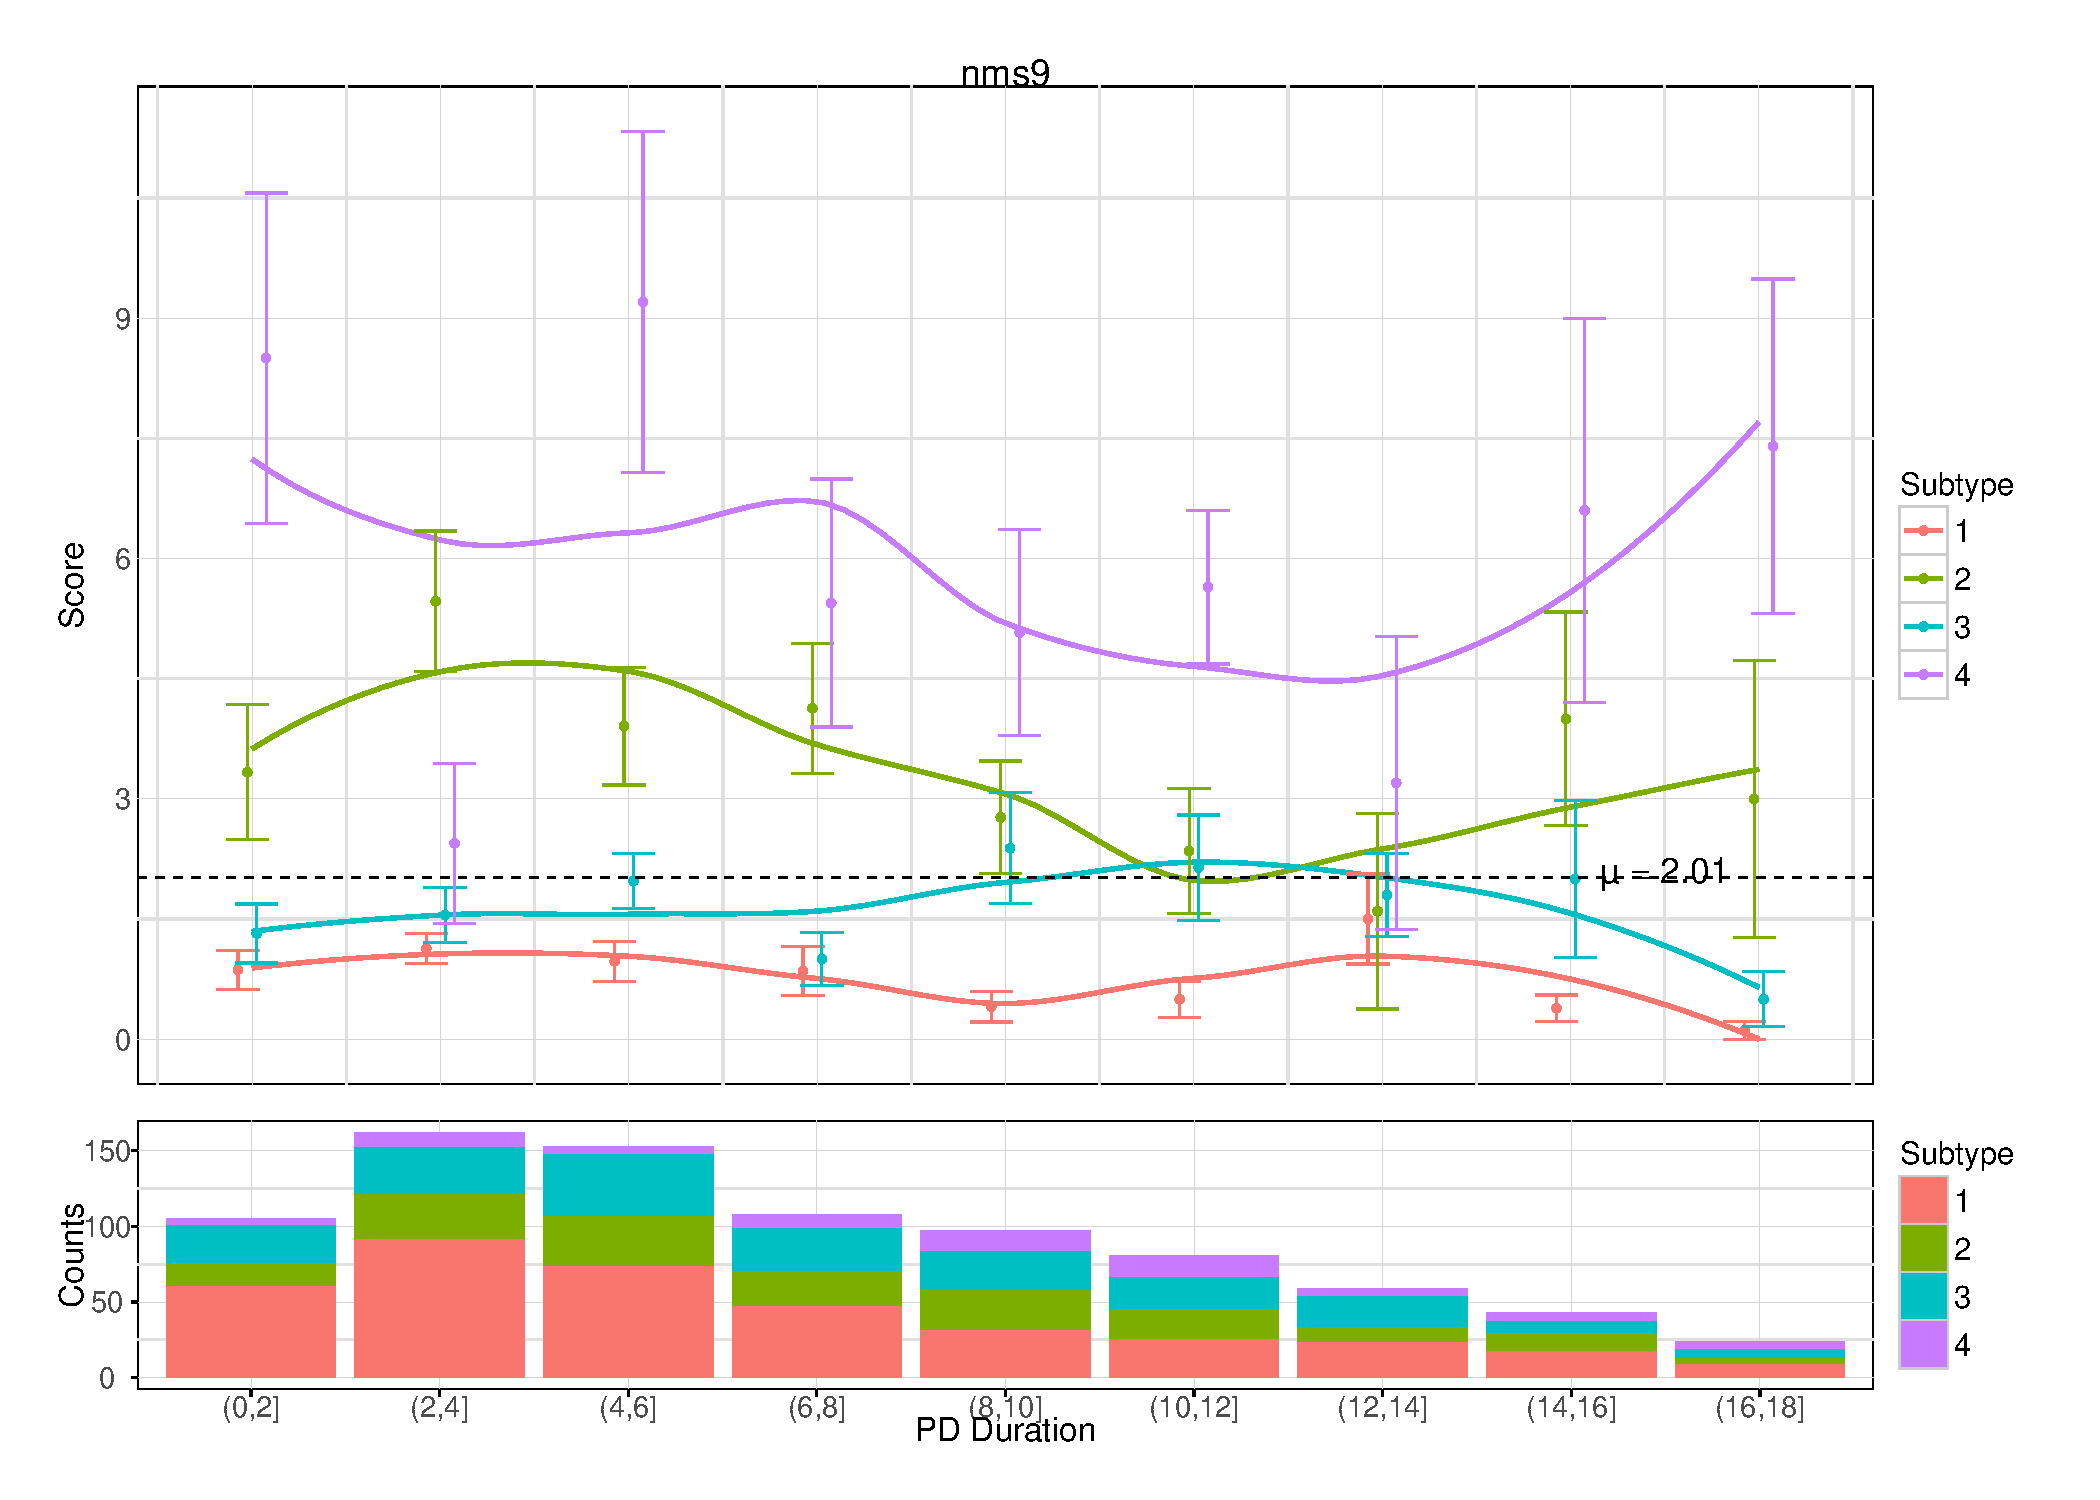
\includegraphics[width=0.8\linewidth]{nms9-multi-durat-counts.pdf}
  \caption{Mean anxiety (nms\_9) score per subtype, with number of patients in each group at
  bottom.}
  \label{fig:nms9-multi}
\end{figure*}

\subsection{Depression}
I plotted the mean nms\_10 (depression) score for each durat\_pd bin in
Figures~\ref{fig:nms10-long} and ~\ref{fig:nms10-multi}.

\begin{figure*}[p]
  \centering
  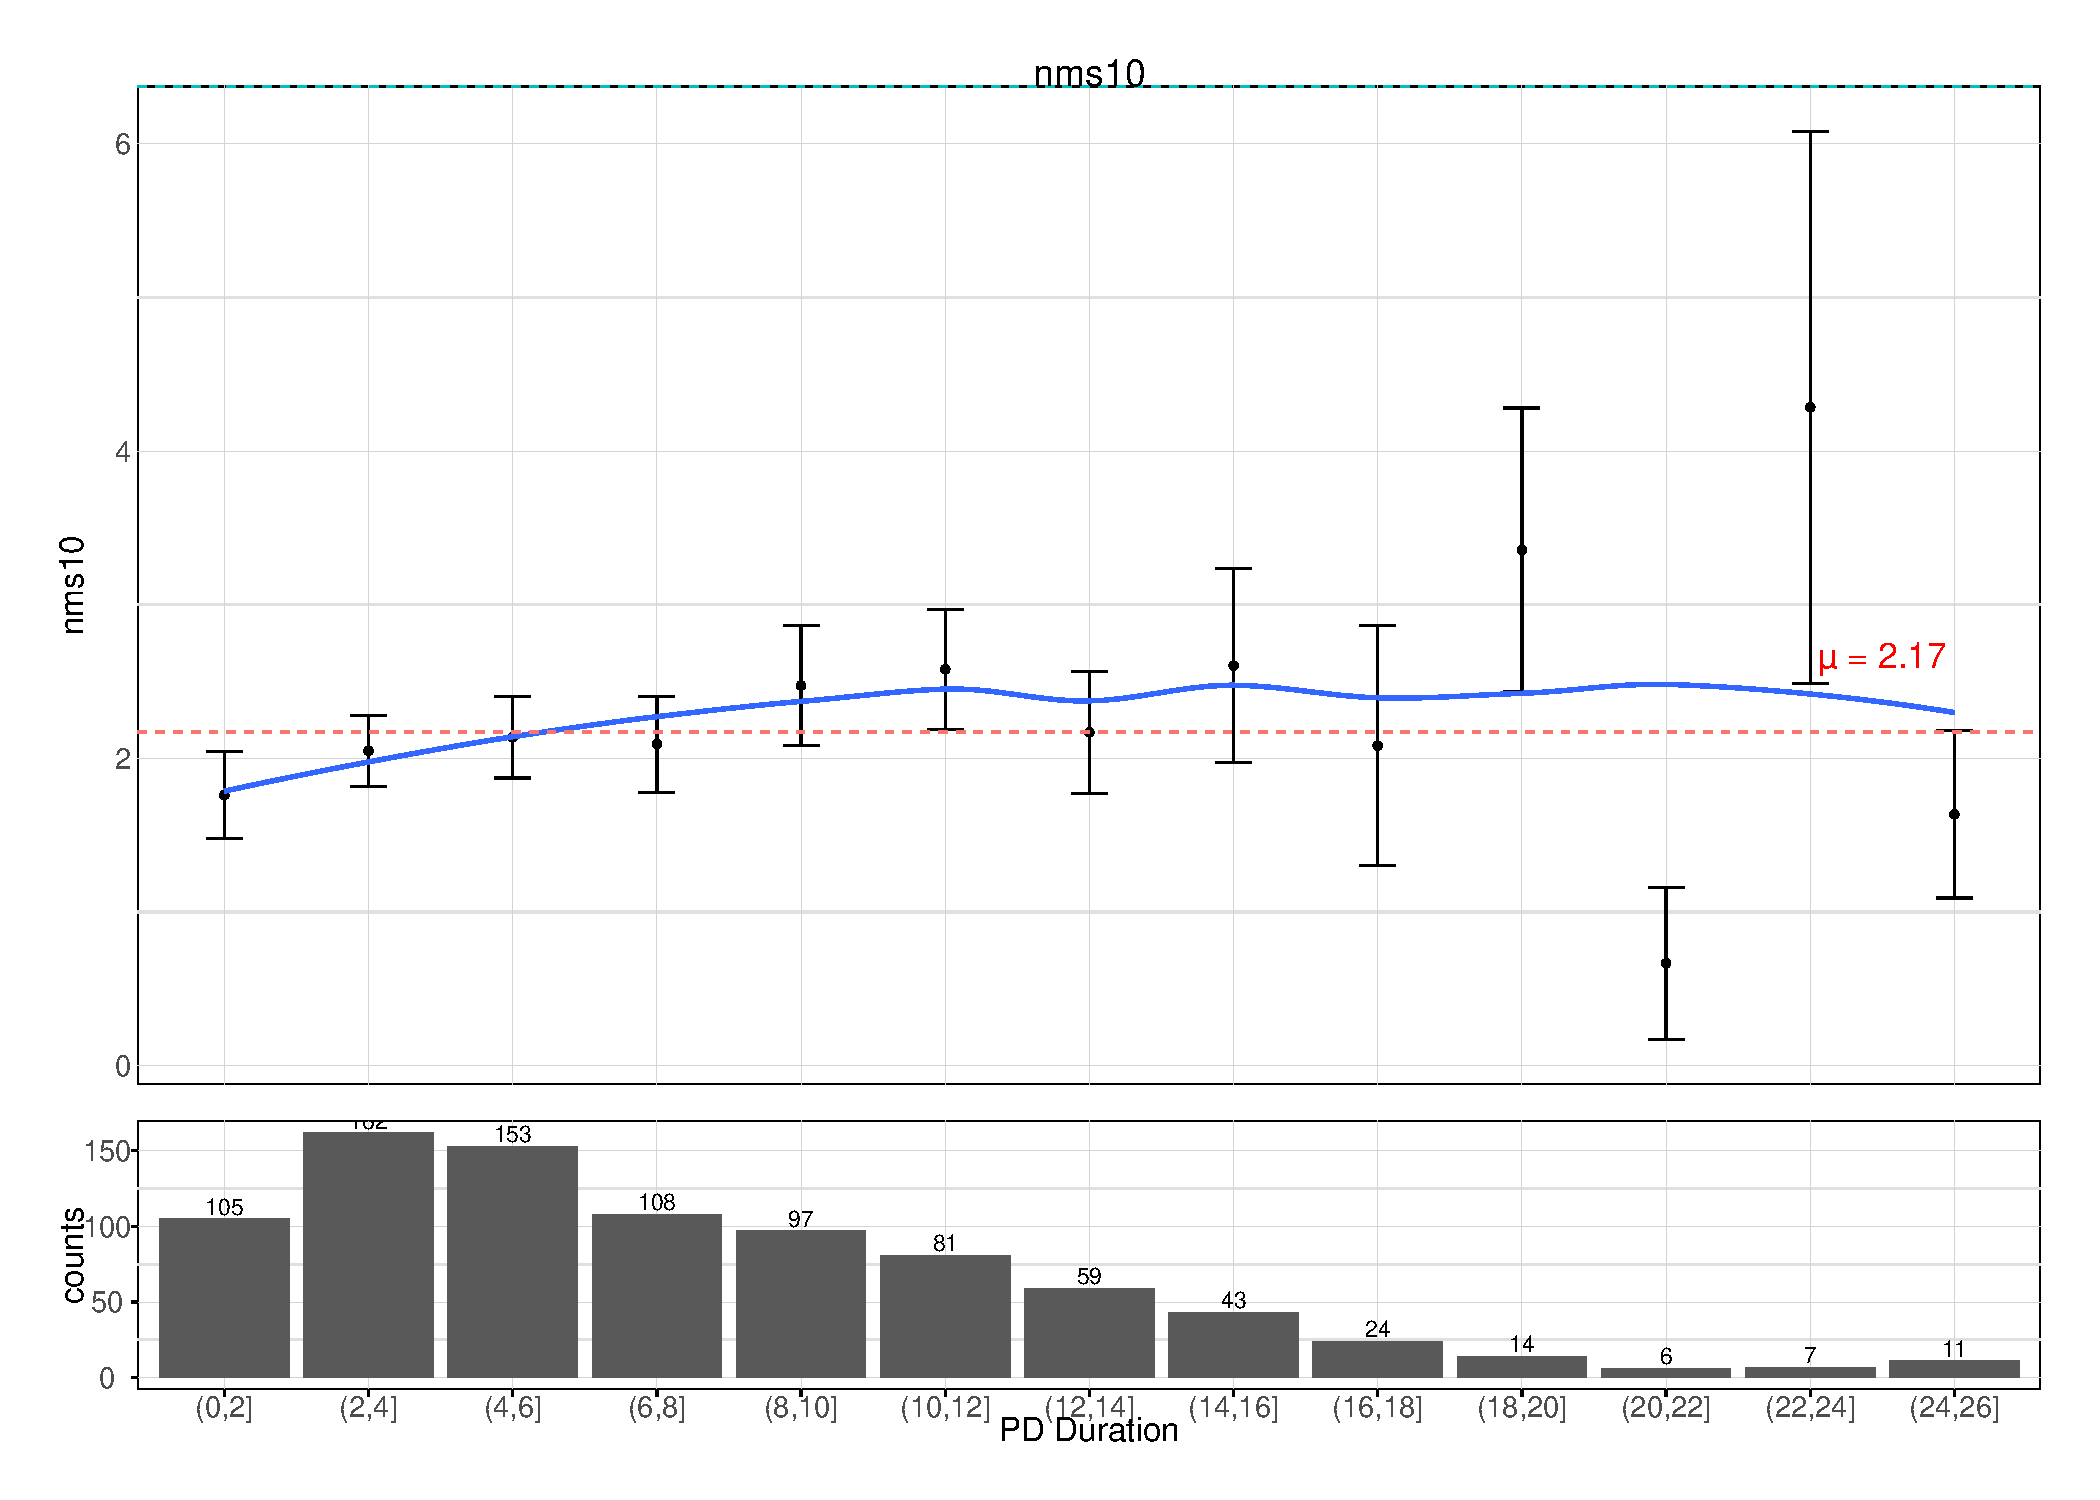
\includegraphics[width=0.8\linewidth]{nms10-durat-counts.pdf}
  \caption{Mean depression (nms\_10) score by PD duration, with number of patients in each group at
  bottom.}
  \label{fig:nms10-long}
\end{figure*}

\begin{figure*}[p]
  \centering
  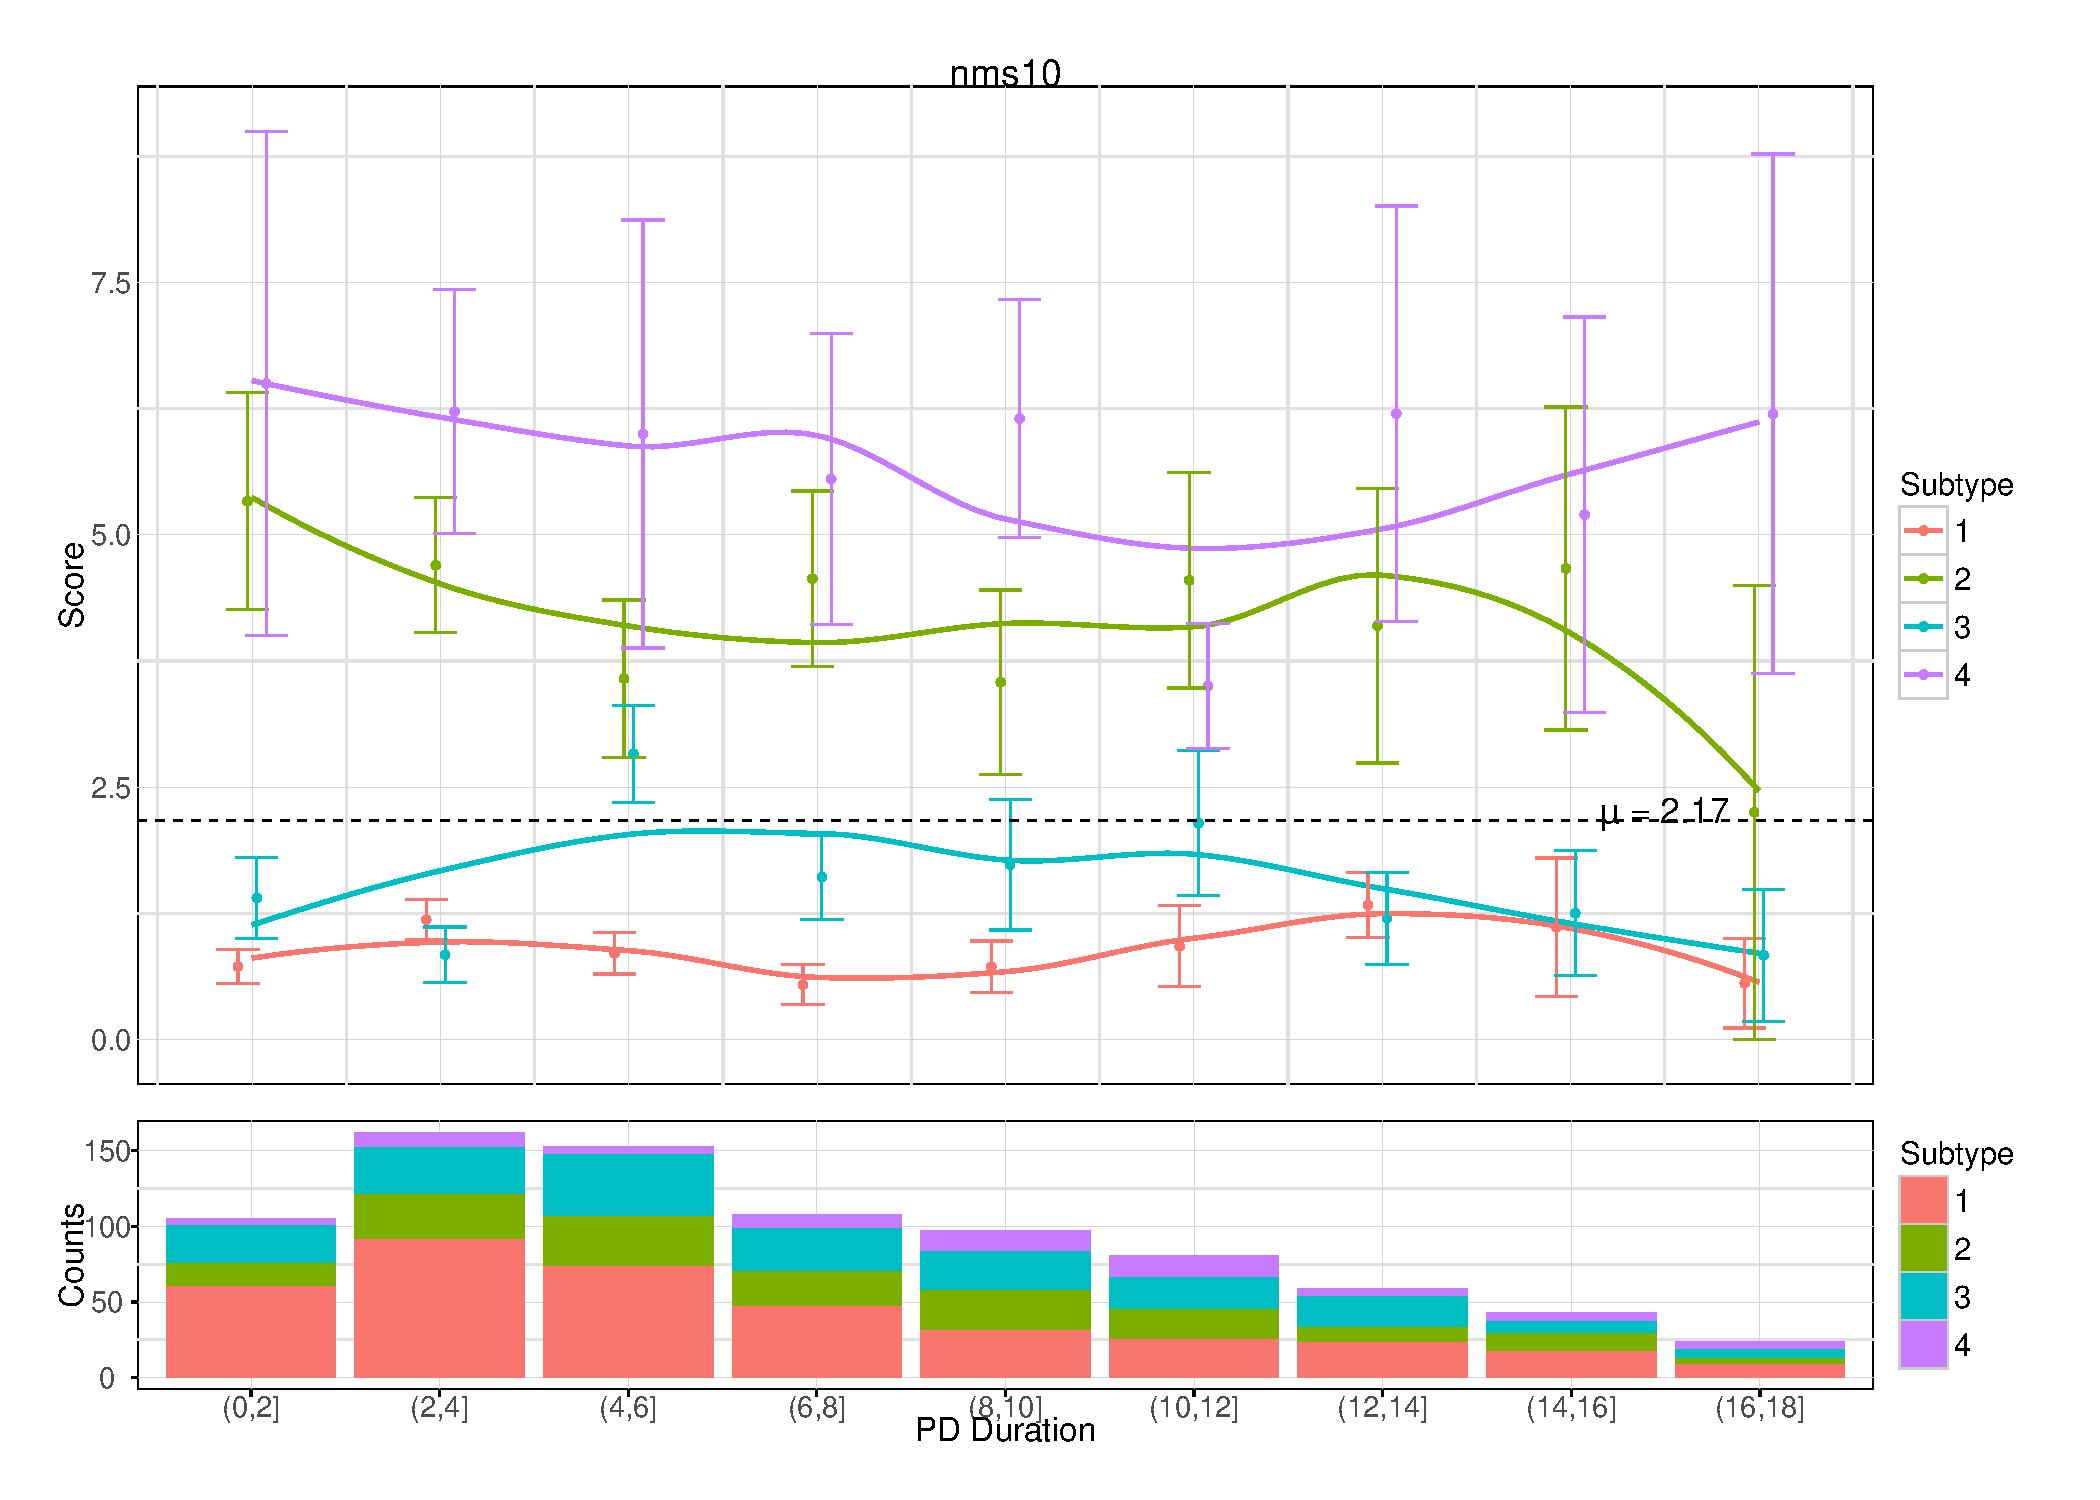
\includegraphics[width=0.8\linewidth]{nms10-multi-durat-counts.pdf}
  \caption{Mean depression (nms\_10) score per subtype, with number of patients in each group at
  bottom.}
  \label{fig:nms10-multi}
\end{figure*}

\subsection{Cisitot}

Note that cisitot has the highest correlation of all of the PD symptoms. I plotted cisitot per
subtype in Figure~\ref{fig:cisitot-multi}. Interestingly, subtypes 2, 3, and 4 generally start from
the same mean motor symptom score, suggesting different paths of disease progression.
% same global mean motor symptom score. % TODO: This is important.

\begin{figure*}[t]
  \centering
  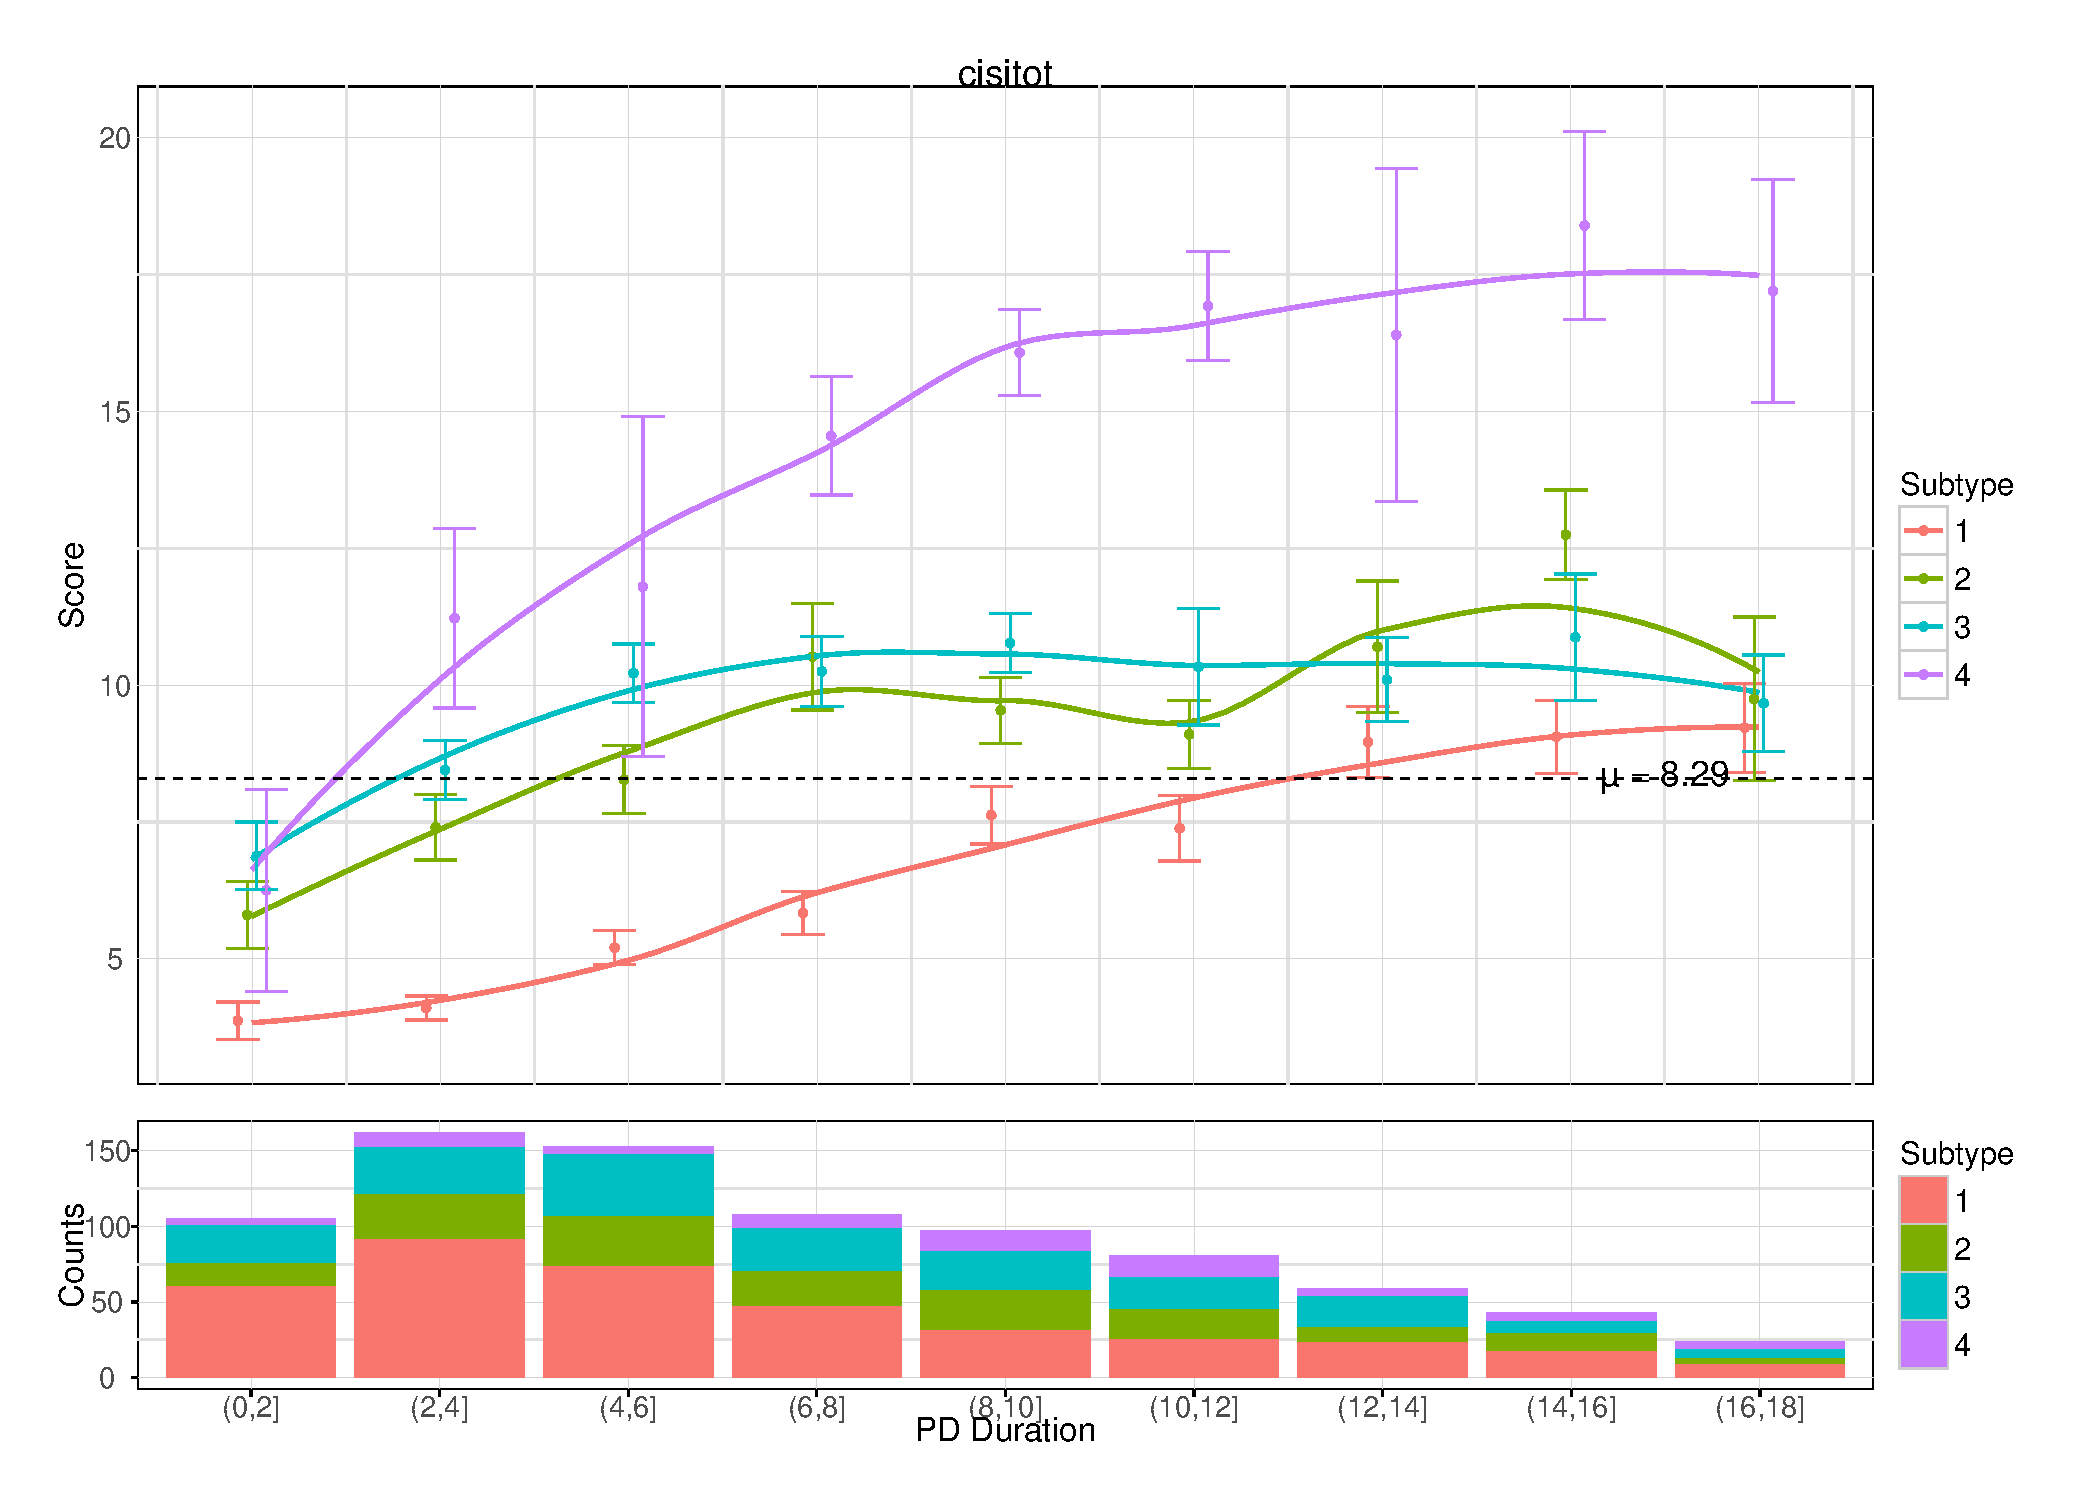
\includegraphics[width=0.8\linewidth]{cisitot-multi-durat-counts.pdf}
  \caption{Mean cisitot score per subtype, with number of patients in each group at
  bottom.}
  \label{fig:cisitot-multi}
\end{figure*}

\subsection{Tremor}

I plotted tremor symptoms in Figure~\ref{fig:tremor-multi}. Notice how in this group, subtype 3
(motor-dom) is higher than all groups towards the beginning of disease progression. This supports
the idea that Subtype 3 is Ma's \cite{ma15} tremor-dominant cluster.

\begin{figure*}[t]
  \centering
  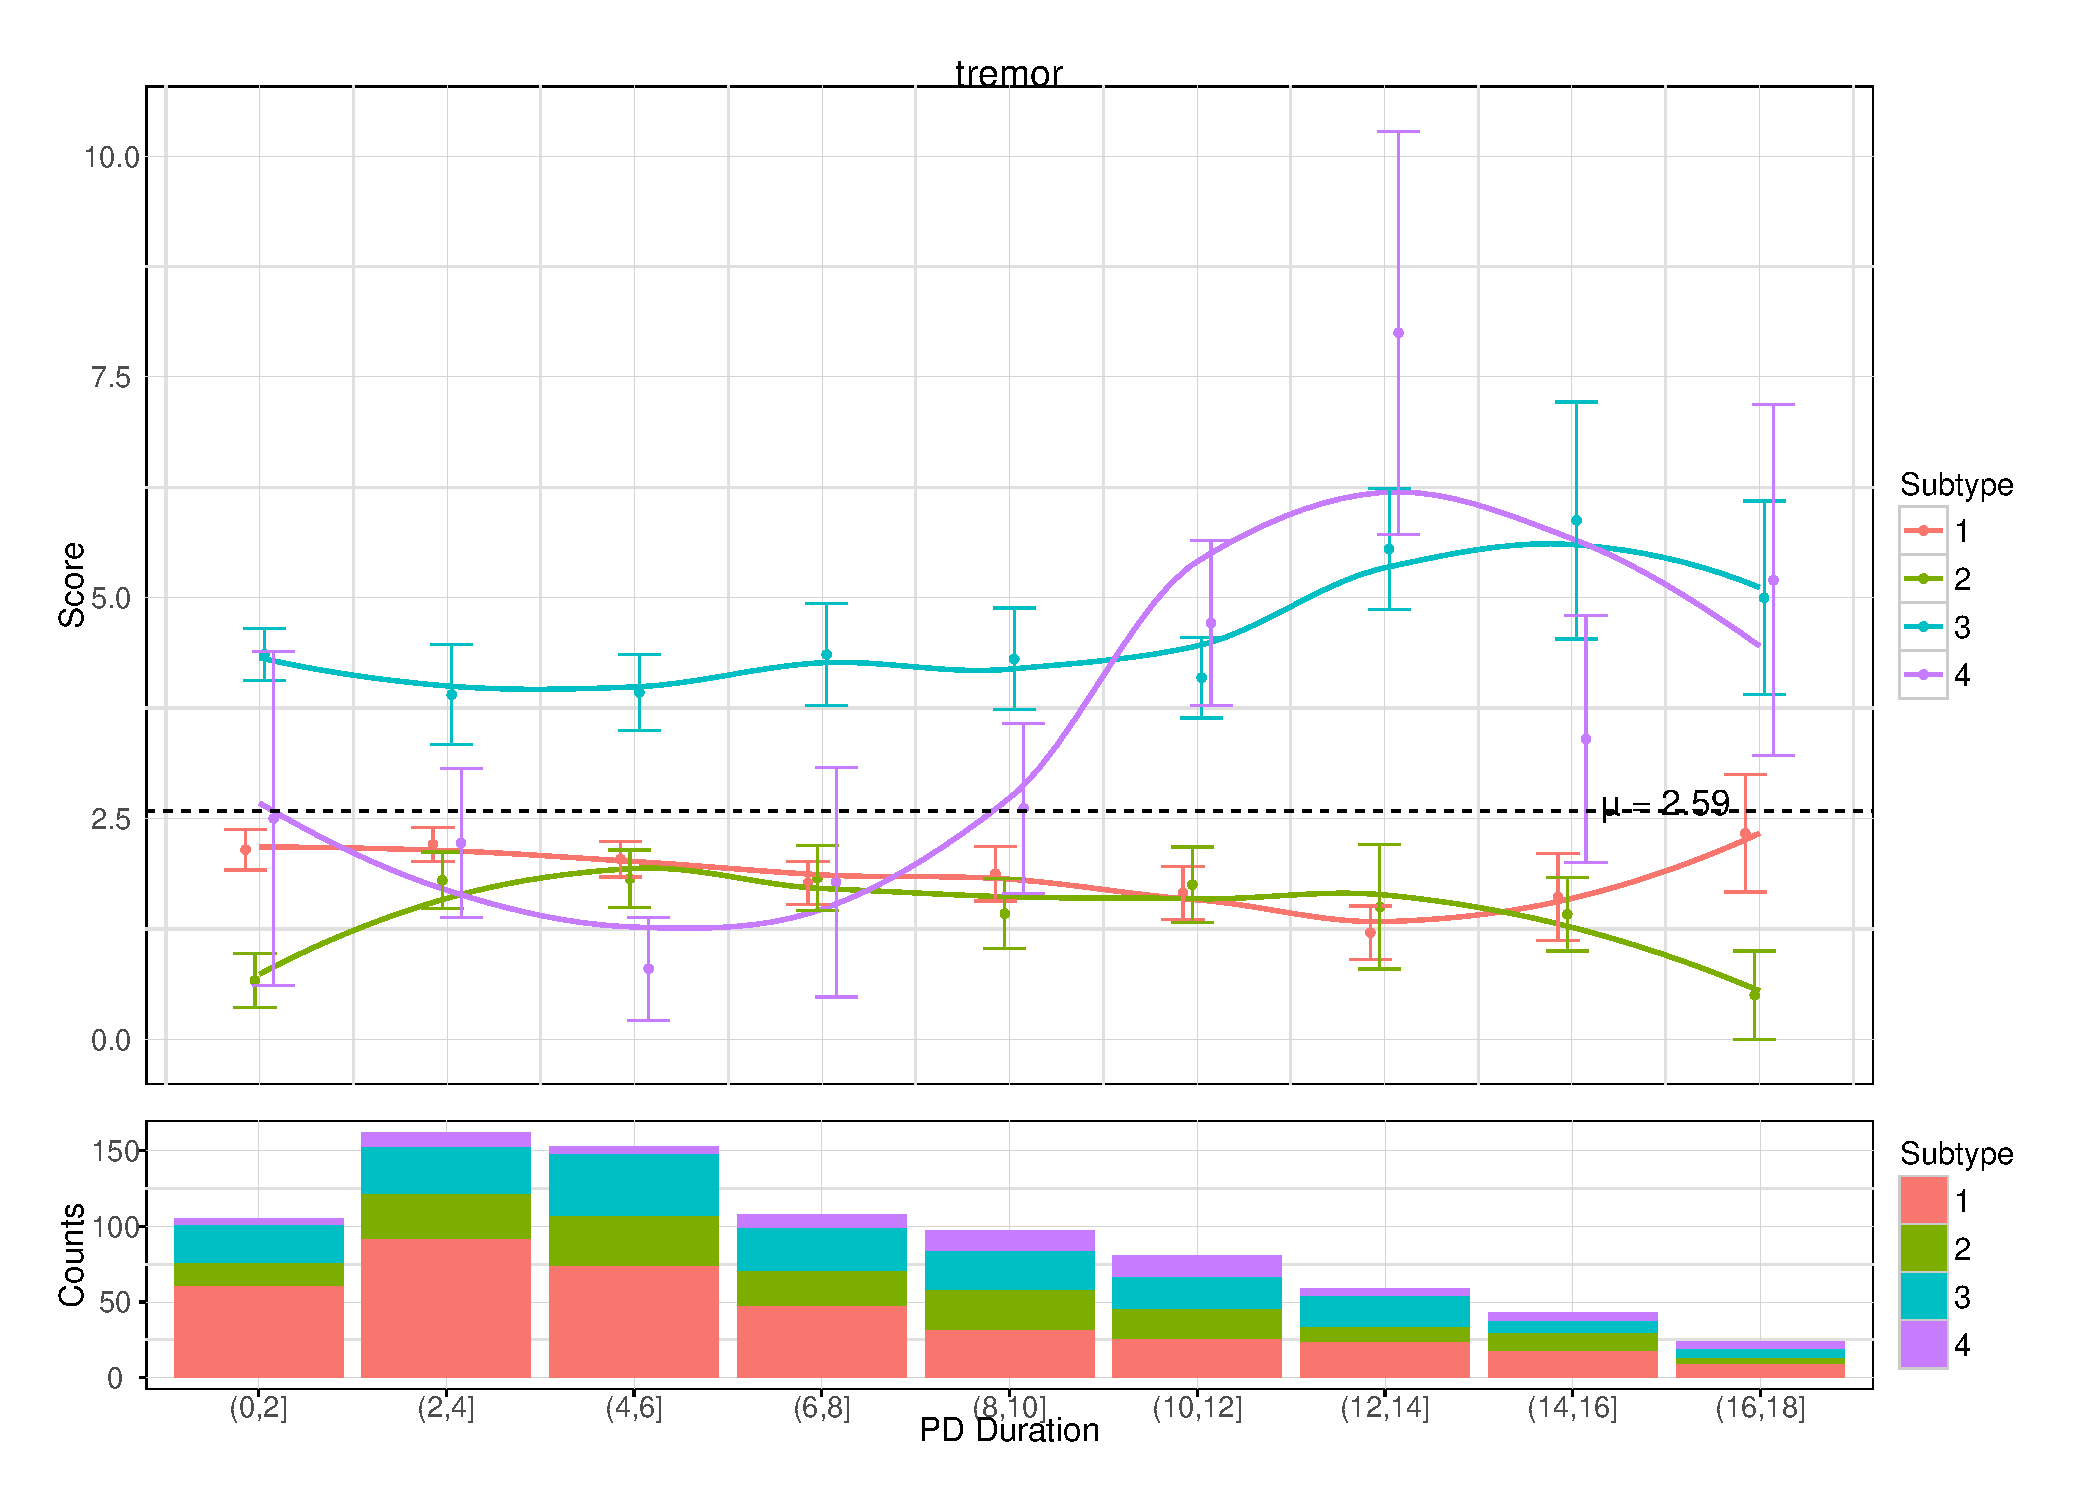
\includegraphics[width=0.8\linewidth]{tremor-multi-durat-counts.pdf}
  \caption{Mean tremor score per subtype, with number of patients in each group at
  bottom.}
  \label{fig:tremor-multi}
\end{figure*}

% TODO: Maybe later
% \subsection{By \texttt{pdonset}}

\section{Extended Nonmotor Symptoms}
\label{sec:nms30}

\subsection{Adding nonmotor symptoms to original $k$-means clustering}

First, I used the clustering with the original 9 nms symptoms, but plotted the original 30 symptoms
instead. The reason for this was to treat the clustering of the 9 symptoms as a form of
dimensionality reduction, since we know each symptom of nms\{1-30\} is colinear with several other
symptoms, and they form the broader nms\_d\{1-9\} symptoms. The results are in
Figure~\ref{fig:d9to30}

\begin{figure*}[p]
  \centering
  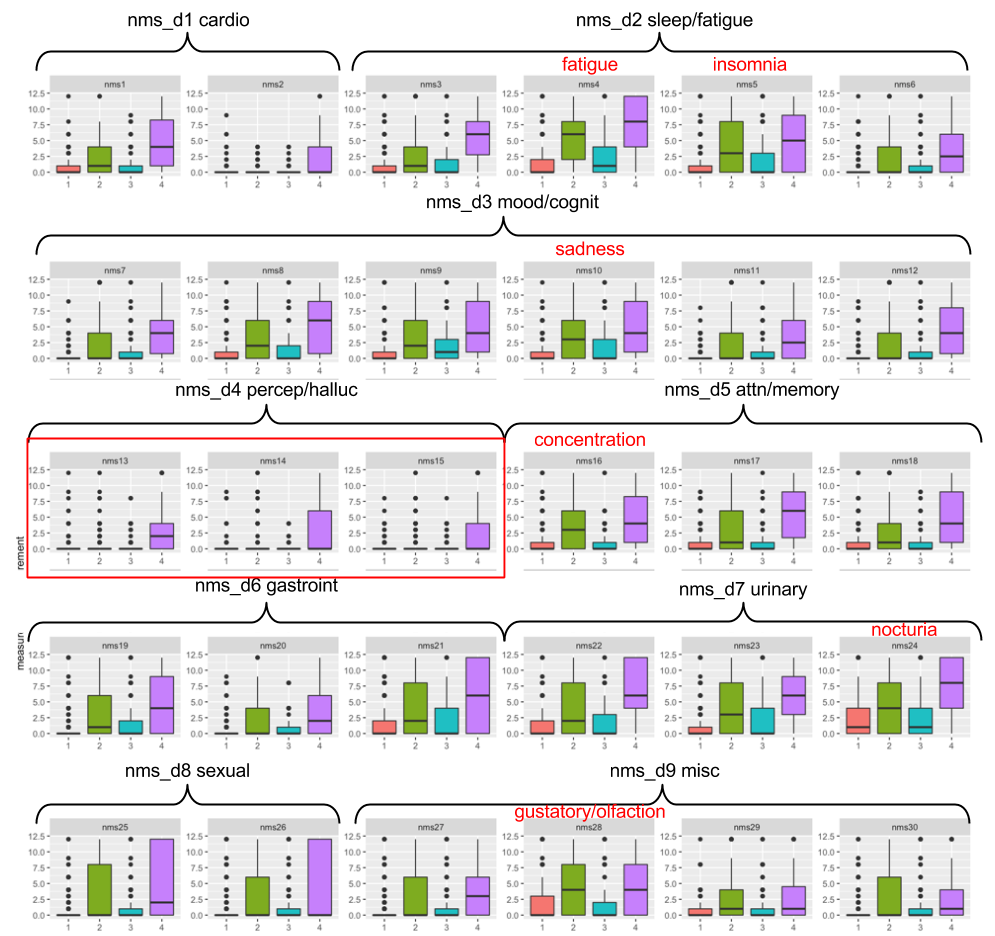
\includegraphics[width=\linewidth]{d9to30.png}
  \caption{All symptoms (nms\{1-30\}) plotted with the original clustering results of the the 9
broader symptoms. Interesting parts of the figure are are labeled in red.}
  \label{fig:d9to30}
\end{figure*}

\subsection{\emph{New} clustering with 30 symptoms}

\subsubsection{Principal Component Analysis}

I ran PCA on the dataset with solely the 30 nonmotor symptoms. A plot of various metrics for
determining the optimal number of eigenvectors is in Figure~\ref{fig:nms30only-eigs}. Most metrics agree
Nthat the optimal number of eigenvalues is around 6, but notice how one component has by far the
highest eigenvalue; this component can be interpreted as a general ``nonmotor severity'' measure,
indicating that much of the general nonmotor symptomatic expression falls along the same dimension.

\begin{figure}[H]
  \centering
  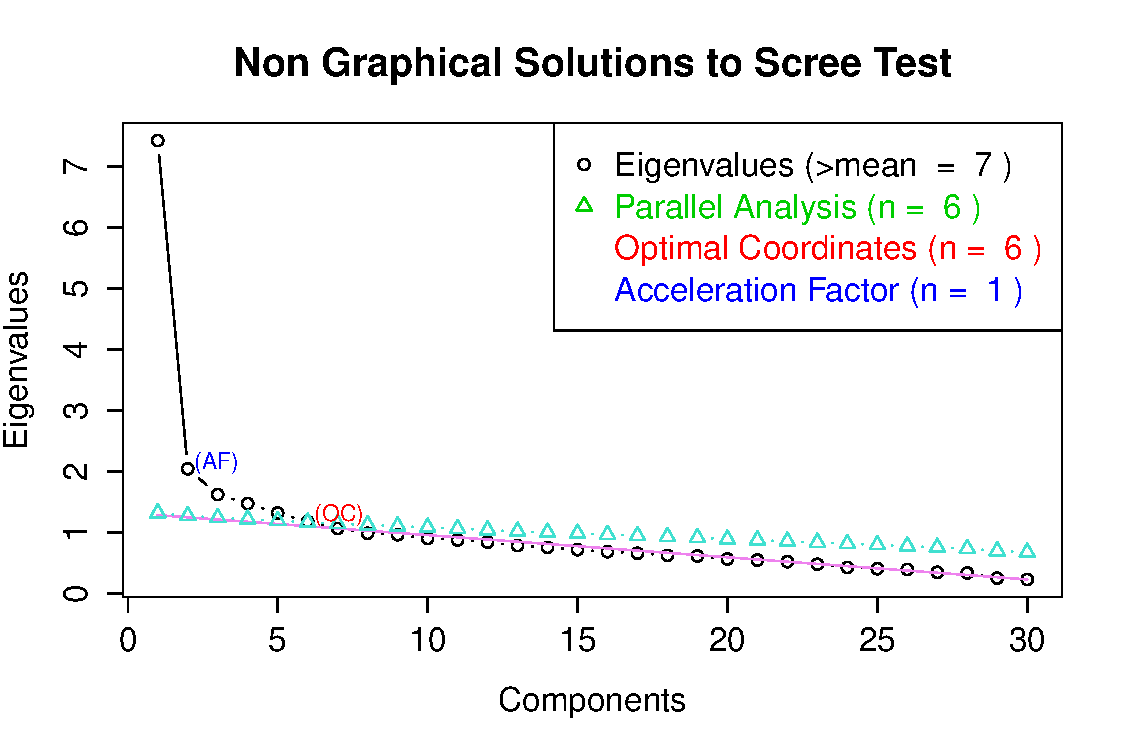
\includegraphics[width=\linewidth]{nms30only-eigs.pdf}
  \caption{Eigenvalues and other metrics for Principal Component Analysis applied to the NMS30 data.}
  \label{fig:nms30only-eigs}
\end{figure}

This principal component can be shown more clearly in the correlation plot of each symptom with the
first 5 components located in Figure~\ref{fig:nms30only-eigscorr}. In the first component, all of the
symptoms have at least a minor positive correlation. The remaining components are composed
primarily of dimensionality reduction in domain 3 (mood/cognition), domain 5 (attention/memory),
domain 7 (urinary), and domain 9 (misc). It is once again demonstrated that mood/cognition symptoms
are very important parts of this dataset.

\begin{figure*}[t]
  \centering
  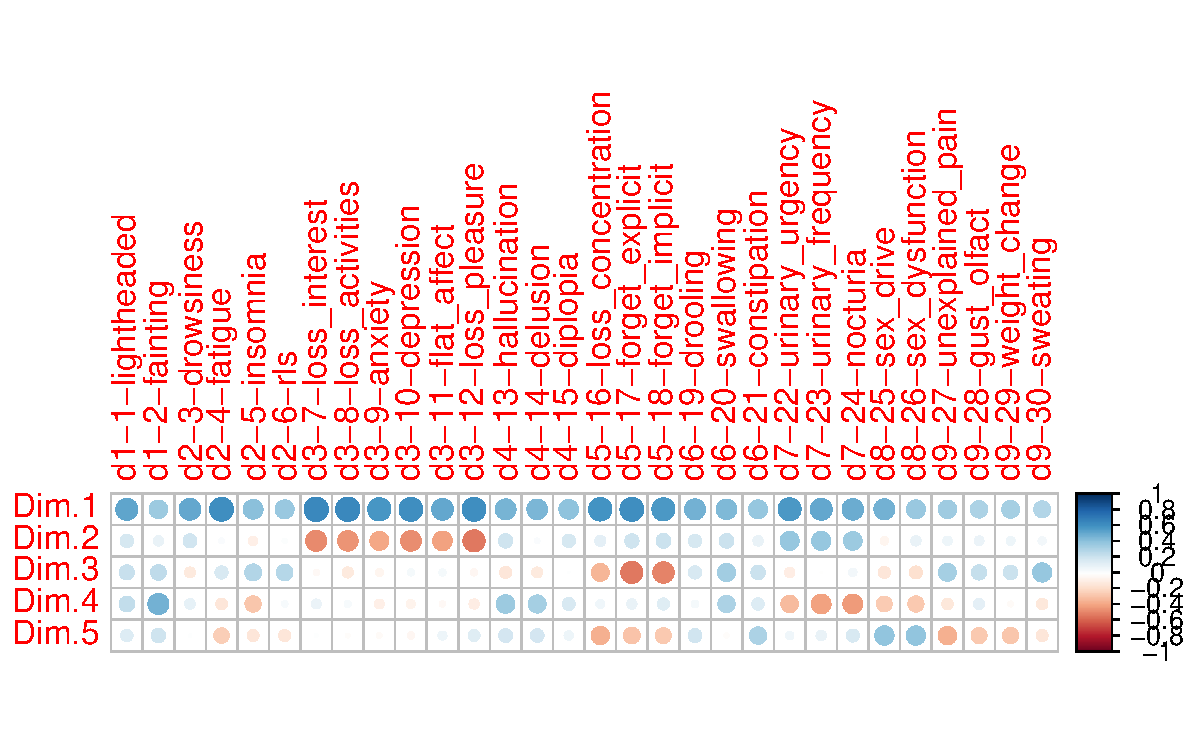
\includegraphics[width=\linewidth]{nms30only-eigscorr.pdf}
  \caption{Correlation of each nonmotor symptom with the first 6 components}
  \label{fig:nms30only-eigscorr}
\end{figure*}

\subsubsection{Symptoms clustering}

\paragraph{Nonmotor only}

I used hierarchical clustering to cluster the 30 symptoms of the dataset using complete linkage.
Results are in Figure~\ref{fig:nms30only-colhc}. Naturally, symptoms that belong to the same domain are
clustered together. But the hierarchical clustering also shows how some symptomatic domains are
closely related; for example, d6 (gastro), d7 (urinary), and d8(sexual). Additionally,
miscellaneous symptoms are quite distinct from the other symptoms.

\begin{figure*}[p]
  \centering
  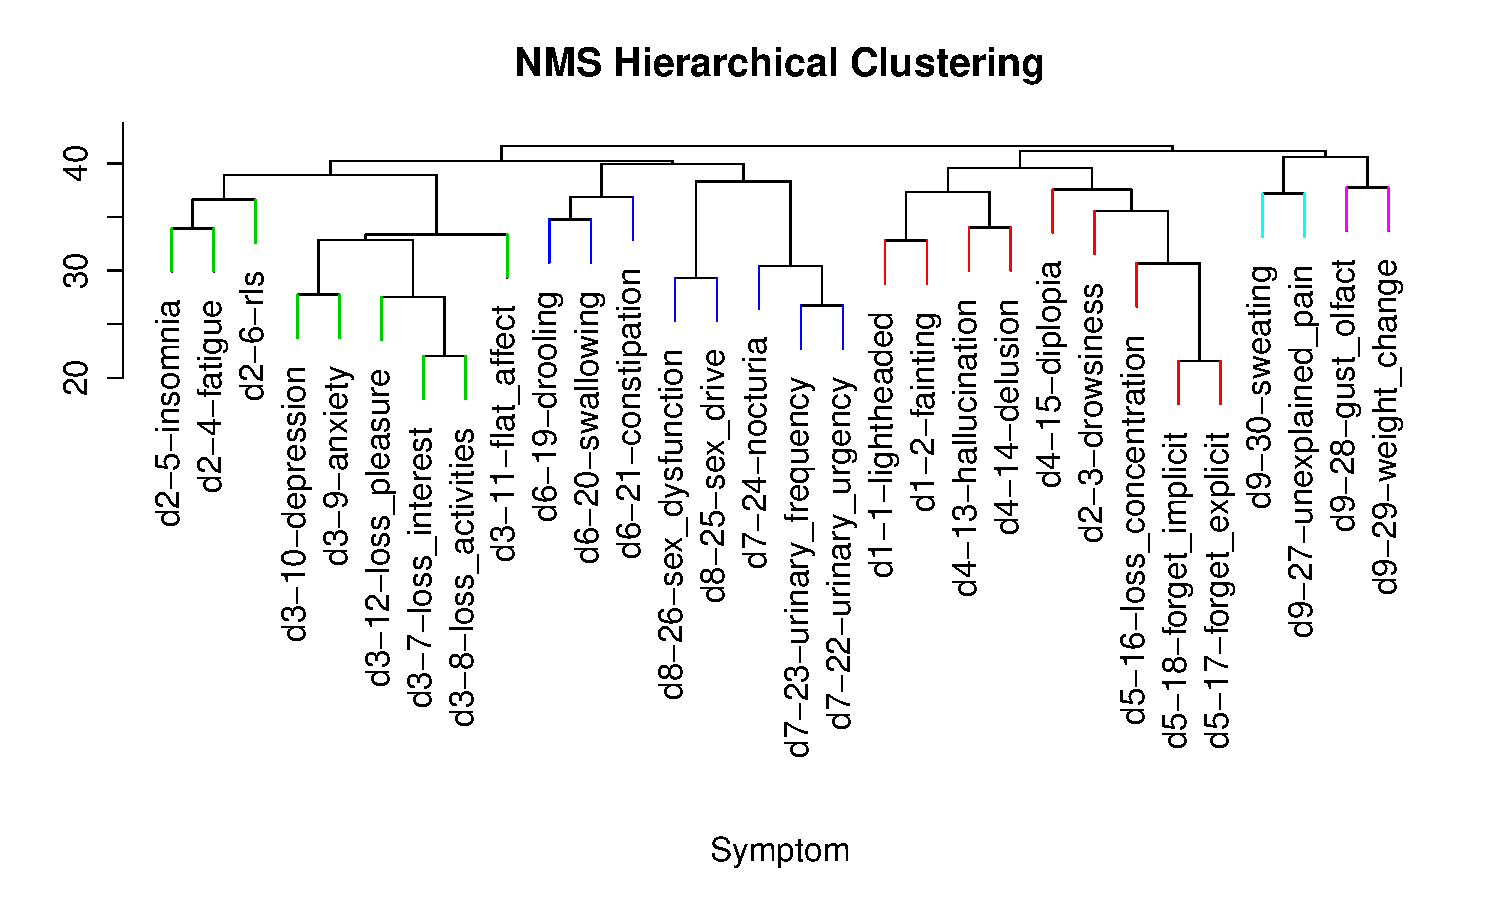
\includegraphics[width=\linewidth]{nms30only-colhc.pdf} \caption{Hierarchical clustering of symptoms.
    Dendrogram colored with 5 clusters. Naming is: d\{1-9\}-\{1-30\}-description}
  \label{fig:nms30only-colhc}
\end{figure*}

\paragraph{With motor symptoms}

In Figure~\ref{fig:nms30m-colhc}, the results are similar to the original hierarchical
clustering; but notice that motor symptoms are clustered together \emph{except} for tremor. In
fact, tremor is the most dissimilar symptom of them all!

\begin{figure*}[p]
  \centering
  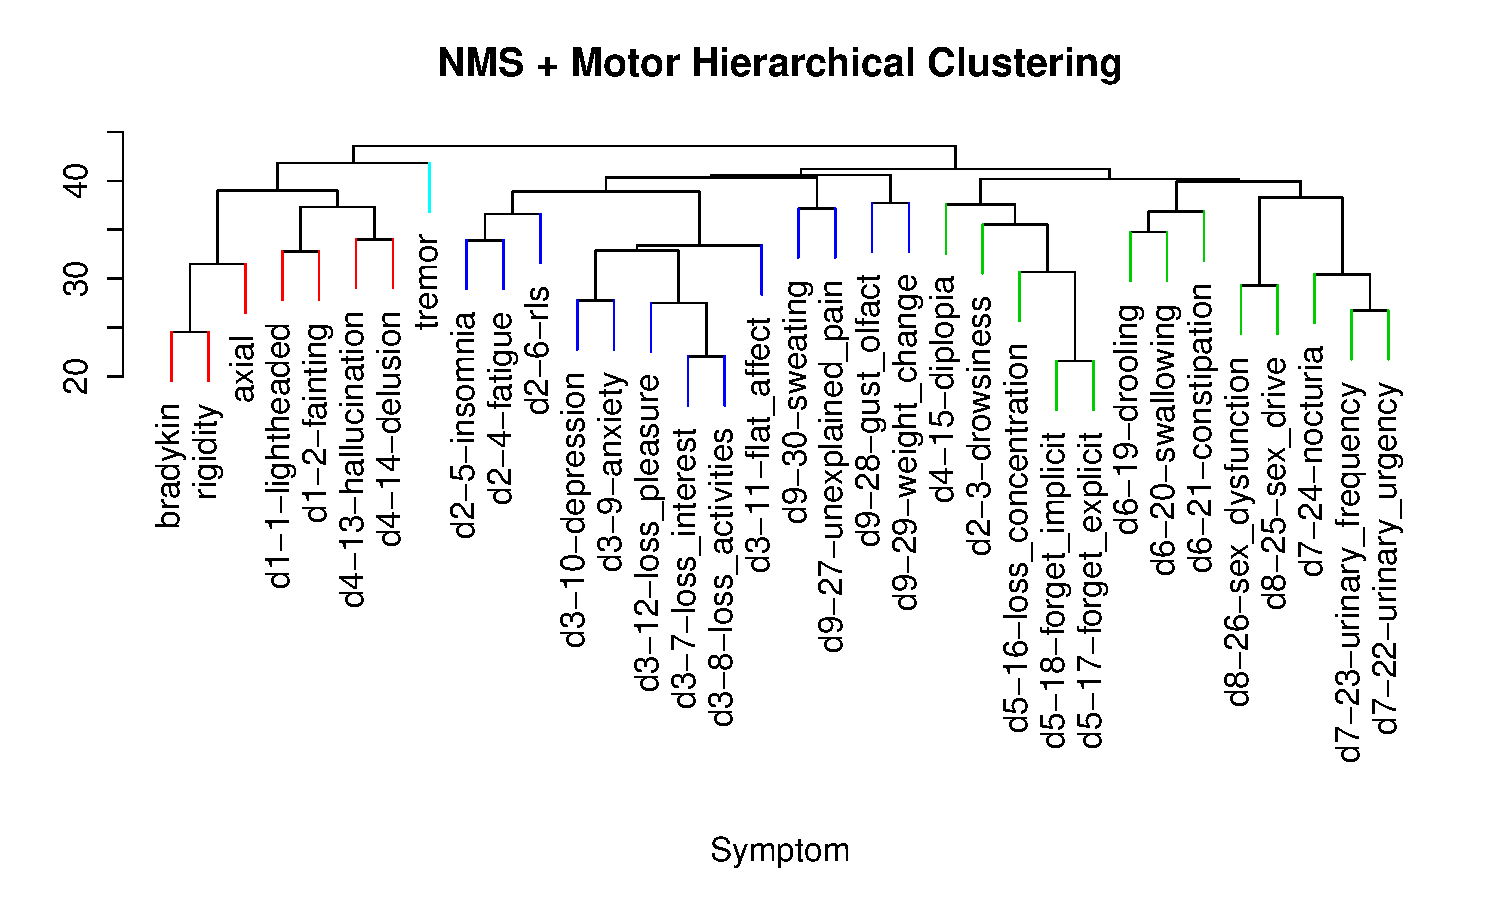
\includegraphics[width=\linewidth]{nms30m-colhc.pdf} \caption{Hierarchical clustering of symptoms
  including motor symptoms.  Dendrogram colored with 4 clusters.}
  \label{fig:nms30m-colhc}
\end{figure*}

\subsubsection{$k$-means}

More so than previously, metrics for identifying the number of clusters proved inconclusive. Most
metrics suggested 2 clusters, which isn't a useful clustering. I decided to stick with $k = 4$ to
compare the results of this new clustering with the previous run. All 30 NMS symptoms were included
as well as the four motor symptoms axial, rigidity, bradykinesia, and tremor.
In this clustering, 4 slightly different subtypes are identified:

\begin{enumerate}
  \item ($n = 509$) Mildly affected in all domains.
  \item ($n = 97$) Higher than average nonmotor symptoms, but severely affected in depressive
    symptoms especially.
  \item ($n = 249$) Averagely affected in all domains.
  \item ($n = 49$) Severely affected in all domains.
\end{enumerate}

Because the number of symptoms is high, I don't provide the boxplots I have previously provided;
instead, I provide a heatmap of $z$-scores in Figure~\ref{fig:nms30m-k4-heatmap-improved} and a
table of results in Table~\ref{tab:nms30_k4}.

\begin{figure*}[p]
  \centering
  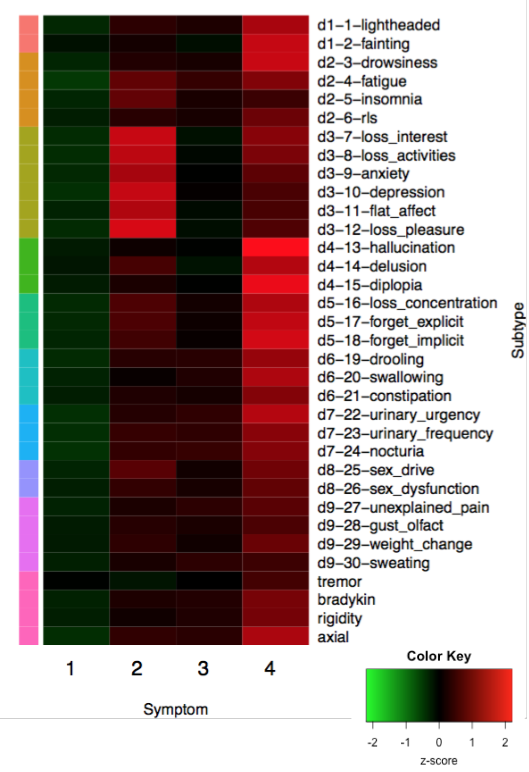
\includegraphics[width=0.6\linewidth]{nms30m-k4-heatmap-improved.png}
  \caption{Heatmap for $k$-means clustering, $k = 4$, with the 30 nonmotor symptoms. Notice that
  subtype 2 is a ``Depression-Dominant'' subtype.} \label{fig:nms30m-k4-heatmap-improved}
\end{figure*}

\begin{table*}[b]
  \centering
  \caption{Mean symptom scores for the centers of the $k$-means clustering where $k = 4$. In
  this case, a Depression-Dominant subtype has been identified.}
  \label{tab:nms30_k4}
  \begin{tabular}{l|l|l|l|l}
cluster & 1 & 2 & 3 & 4 \\
\hline
d1-1-lightheaded & 2.08 & 2.43 & 0.55 & 5.18 \\
d1-2-fainting & 0.17 & 0.53 & 0.13 & 2.45 \\
d2-3-drowsiness & 2.51 & 2.77 & 0.97 & 7 \\
d2-4-fatigue & 4.84 & 6.29 & 1.3 & 7.31 \\
d2-5-insomnia & 3.16 & 5.46 & 1.2 & 4.22 \\
d2-6-rls & 1.88 & 2.31 & 0.66 & 3.88 \\
d3-7-loss\_interest & 1.04 & \textbf{6.08} & 0.41 & 4.59 \\
d3-8-loss\_activities & 1.7 & \textbf{7.14} & 0.7 & 5.37 \\
d3-9-anxiety & 1.97 & \textbf{6.63} & 0.91 & 4.57 \\
d3-10-depression & 2.35 & \textbf{7.81} & 0.81 & 4.29 \\
d3-11-flat\_affect & 0.91 & \textbf{4.95} & 0.39 & 2.71 \\
d3-12-loss\_pleasure & 1.09 & \textbf{6.82} & 0.36 & 3.43 \\
d4-13-hallucination & 0.58 & 0.82 & 0.2 & 4.63 \\
d4-14-delusion & 0.16 & 1.49 & 0.11 & 3.14 \\
d4-15-diplopia & 0.56 & 1.01 & 0.16 & 4.39 \\
d5-16-loss\_concentration & 2.47 & 4.02 & 0.91 & 6.55 \\
d5-17-forget\_explicit & 2.18 & 3.77 & 0.86 & 6.69 \\
d5-18-forget\_implicit & 1.76 & 3.12 & 0.68 & 6.65 \\
d6-19-drooling & 3 & 2.99 & 0.67 & 6.1 \\
d6-20-swallowing & 1.74 & 1.24 & 0.37 & 4.53 \\
d6-21-constipation & 3.31 & 3.63 & 1.65 & 6.96 \\
d7-22-urinary\_urgency & 3.84 & 3.49 & 0.99 & 7.8 \\
d7-23-urinary\_frequency & 3.79 & 3.98 & 0.94 & 6.51 \\
d7-24-nocturia & 5.13 & 4.99 & 1.67 & 7.65 \\
d8-25-sex\_drive & 2.34 & 4.46 & 0.76 & 5.16 \\
d8-26-sex\_dysfunction & 2.39 & 3.21 & 0.79 & 4.61 \\
d9-27-unexplained\_pain & 2.98 & 2.48 & 0.7 & 4.24 \\
d9-28-gust\_olfact & 3.18 & 3.57 & 1.49 & 4.73 \\
d9-29-weight\_change & 1.86 & 2.54 & 0.88 & 3.92 \\
d9-30-sweating & 2.77 & 2.2 & 0.68 & 3.18 \\
\hline
tremor & 2.59 & 2.12 & 2.53 & 4.1 \\
bradykin & 2.83 & 2.76 & 1.98 & 3.86 \\
rigidity & 2.61 & 2.42 & 1.87 & 3.61 \\
axial & 4.22 & 4.4 & 2.17 & 7.24 \\
  \end{tabular}
\end{table*}

\subsubsection{Model-based expectation-maximization}

Because the dimensionality is quite high in this case; $k$-means may not have provided particularly
accurate results; thus, I tried using a Gaussian mixture model-based clustering package. Various
models were tried, with Bayesian Information Criterion (BIC) plotted in
Figure~\ref{fig:nms30m-bic}. The best
fitting model(s) that maximized the Bayesian Information Criterion include the diagonal, varying
volume, equal shape Gaussian mixture model (VEI) at 11 clusters and the ellipsoidal, equal shape
model (VEV) with 3 clusters. However, the VEV model wasn't interesting; it simply partitioned
individuals into low, medium, and high overall severity.

\begin{figure}[H]
  \centering
  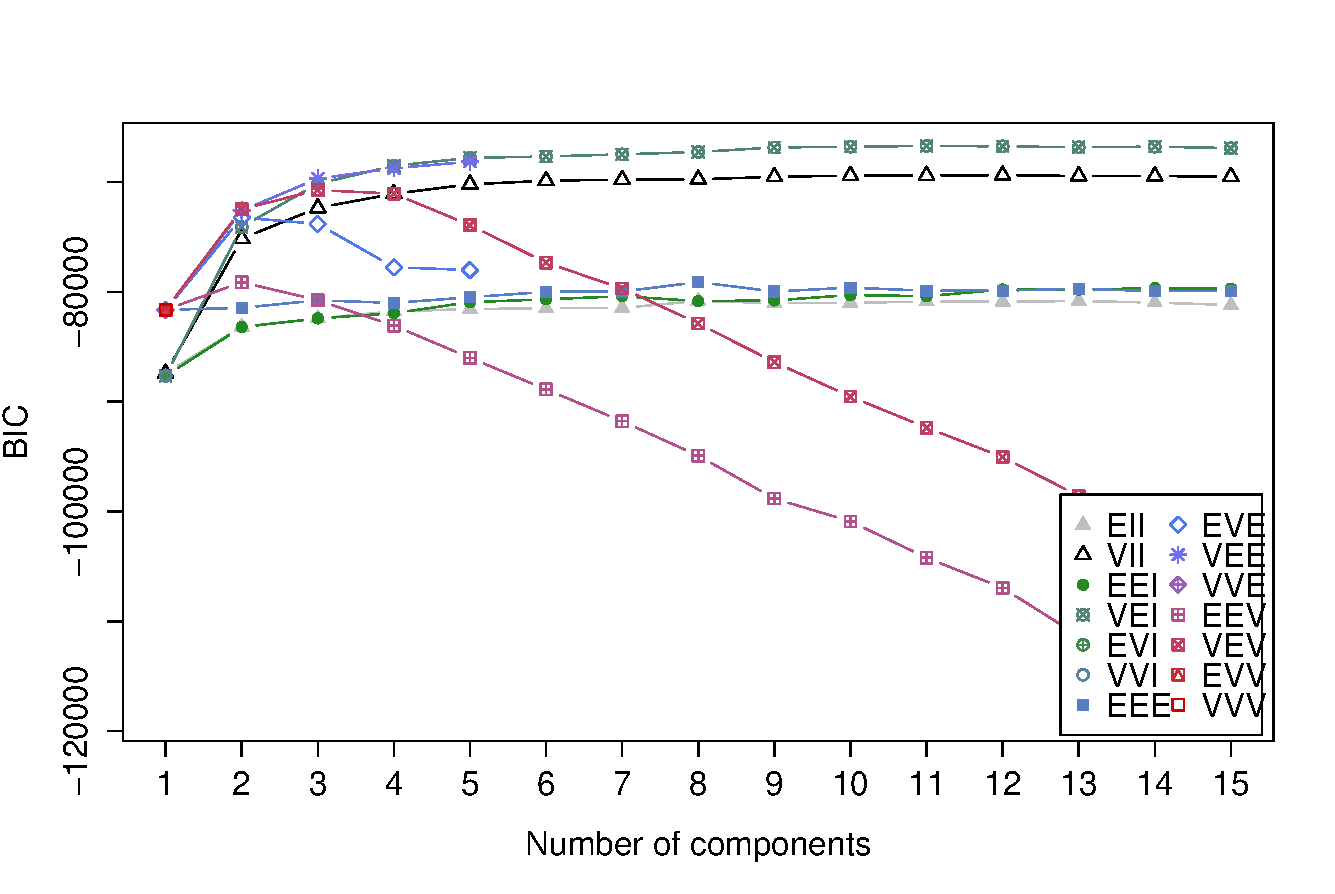
\includegraphics[width=\linewidth]{nms30m-bic.pdf}
  \caption{Bayesian Information Criterion for various Gaussian mixture models, plotted against the
  number of clusters in each model. The best model found is the diagonal, varying volume, equal
shape Gaussian mixture model (VEI) at 11 clusters; notice also that the ellipsoidal, equal shape
model (VEV) is able to achieve a relatively high BIC with only 3 clusters. The VEV model, however,
is not particularly informative.}
  \label{fig:nms30m-bic}
\end{figure}

The VEI model, with 11 clusters, is more interesting. There are many clusters in the data that are
expected, including a few generally mild clusters and a few generally severe clusters.  But, by
isolating more ``interesting'' clusters, we begin to see smaller, more specific proportions of PD
patients. These clusters seem to clarify and expand upon the results found in previous analyses.
The clusters, summarized, are:

\begin{itemize}
  \item[1-3.] ($n = 41,\; 77,\; 150$) Mild in all domains. Cluster 1 is especially mild in motor
    symptoms (see cisitot).
  \item[4.] ($n = 38$) Insomnia-dominant.
  \item[5.] ($n = 43$) Motor-dominant.
  \item[6.] ($n = 163$) Average.
  \item[7.] ($n = 54$) Urinary-dominant.
  \item[8.] ($n = 177$) Above-average in all domains.
  \item[9.] ($n = 67$) Depression-dominant.
  \item[10.] ($n = 81$) Nonmotor-dominant.
  \item[11.] ($n = 13$) Severe in all domains.
% 1	2  3	4   5  6    7  8    9   10  11
% 41  77 150  38  43 163  54 177  67  81  13
\end{itemize}

A heatmap of all 11 clusters found is located in Figure~\ref{fig:nms30m-mclust-heatmap-improved}.

\begin{figure*}[p]
  \centering
  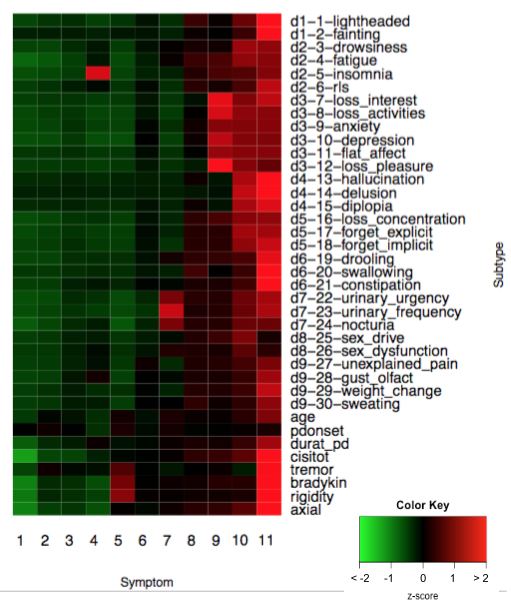
\includegraphics[width=0.7\linewidth]{nms30m-mclust-heatmap-improved.png}
  \caption{Heatmap of clusters found using the VEI Gaussian Mixture Model.}
  \label{fig:nms30m-mclust-heatmap-improved}
\end{figure*}

\subsection{Decision Trees}

I created decision trees for the $k$-means $k = 4$ clustering, located in
Figure~\ref{fig:nms30m-dtree-all}

\begin{figure*}[p]
  \centering
  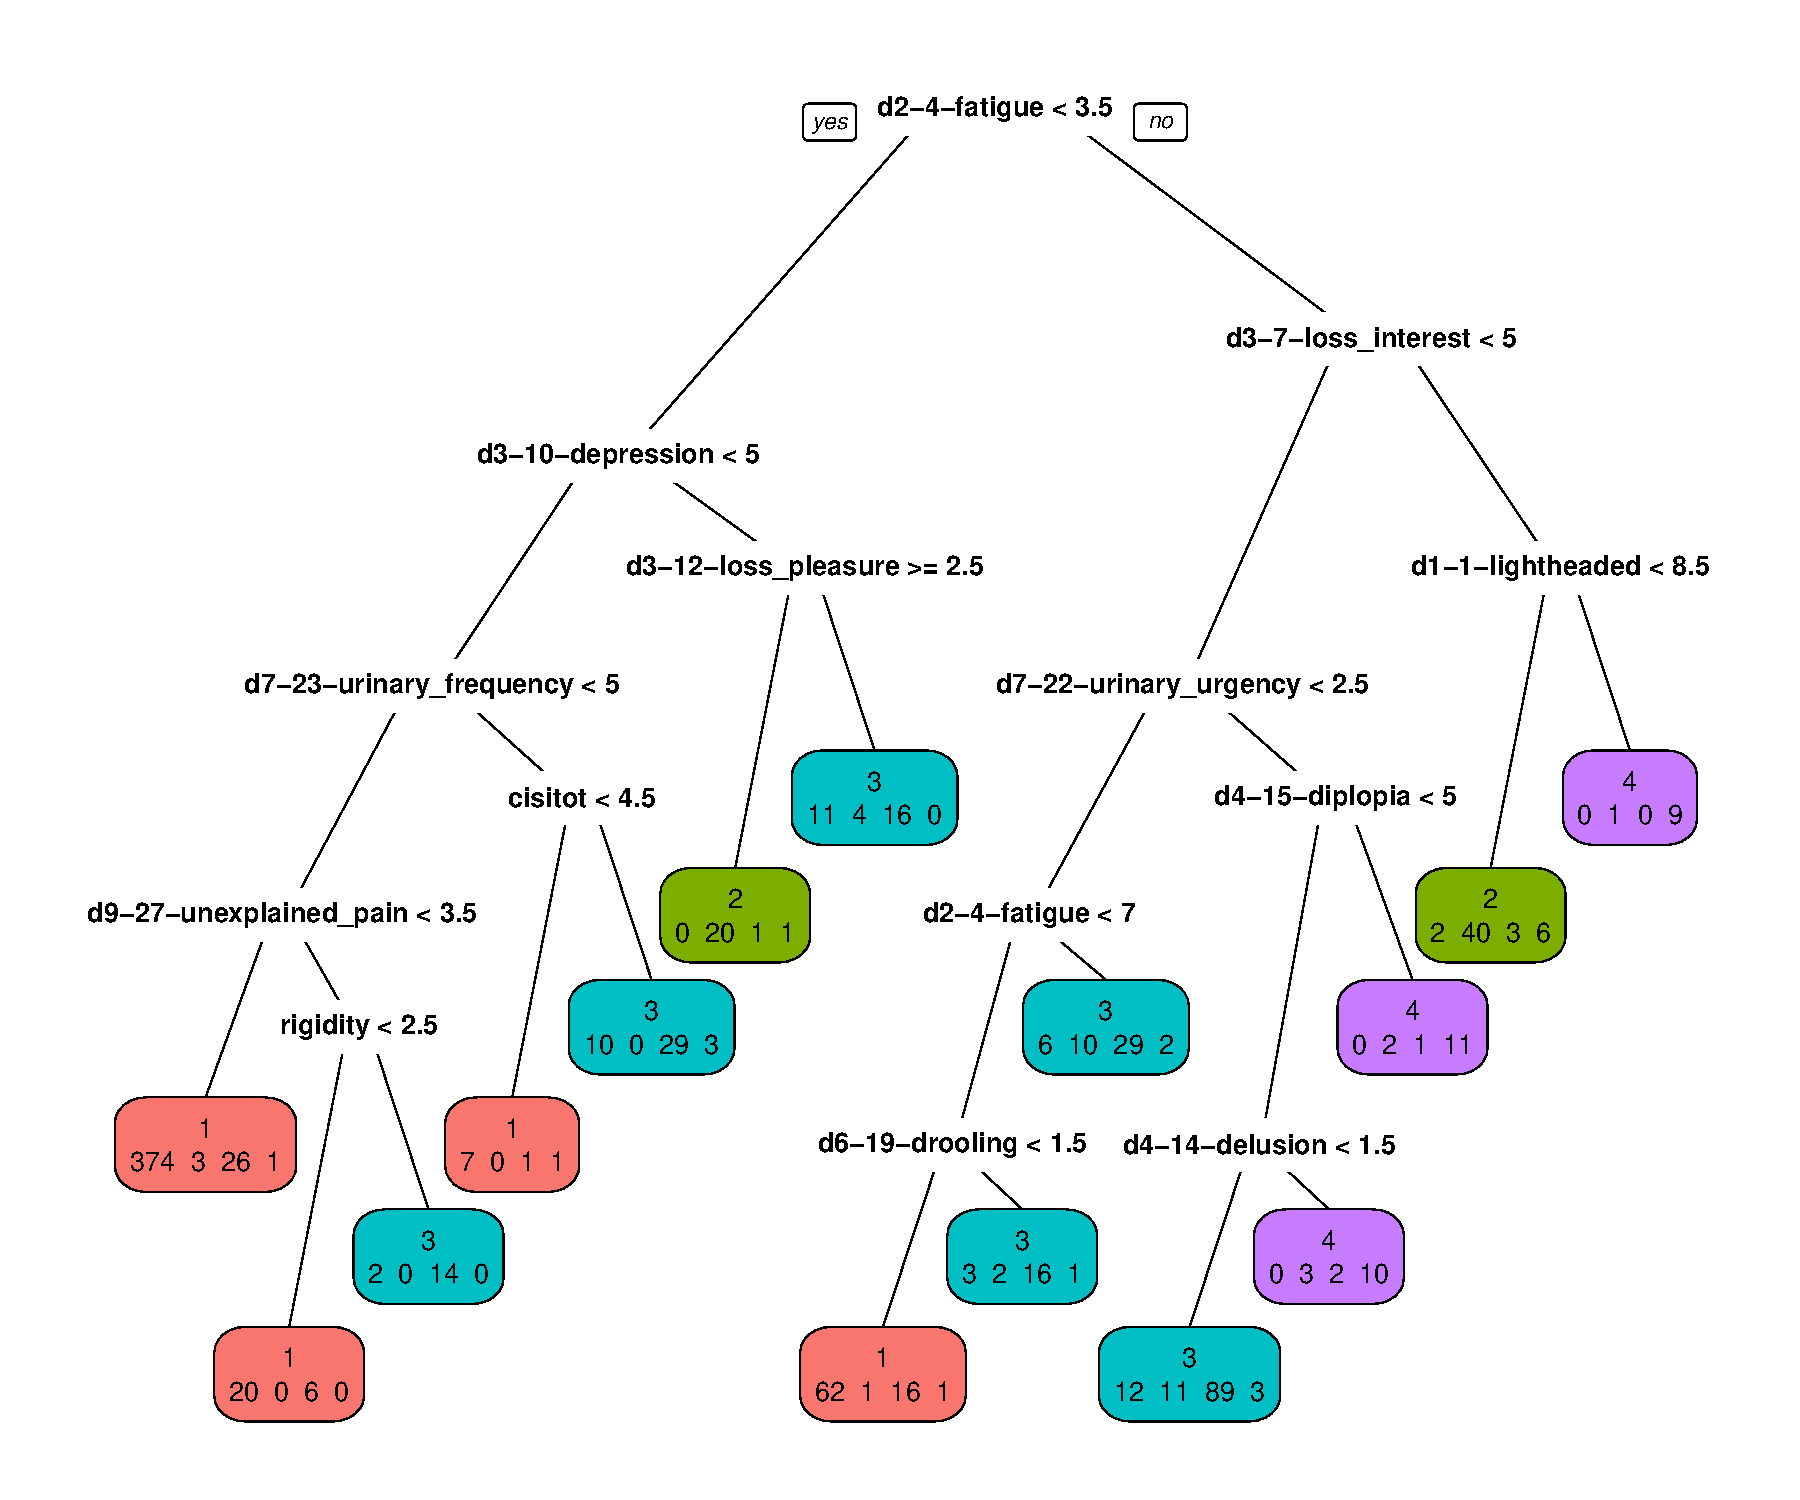
\includegraphics[width=\linewidth]{nms30m-dtree-all.pdf}
  \caption{Pruned decision tree for one vs all, clustered on nms\{1-30\}}
  \label{fig:nms30m-dtree-all}
\end{figure*}

\section{Preliminary Conclusions}

\subsection{Overall clustering}
$k$-means clustering on this Parkinsons' Disease data set reveals clusters that confirm previous
findings in the field, mainly van Rooden et al. \cite{vanrooden10} and the identification of four
subtypes of Parkinson's disease: mild, nonmotor-predominant, motor-predominant, and severe.  van
Rooden's work was done with a separate dataset using a different modeling method
(expectation-maximization), and this investigation independently confirms these subtype
classifications. Unlike van Rooden, mean disease durations differences do exist between subtypes 1
(mild) and 4 (severe), likely due to further development of the disease, although the differences
between 2 and 3 (nonmotor/motor predominated) subtypes are insignificant
(Table~\ref{tab:tukeyhsd}), suggesting different developmental paths of the disease.

Overall, little information was found in pdonset,
durat\_pd, or current age, according to Tables~\ref{tab:tukeyhsd}
and~\ref{tab:info_gain}.  Mean ages were similar for subgroups 1, 2, and 3 ($p >
0.05$, but different for the severe subtype 4, which makes sense given that
patients in 4 also have longer disease durations. Specifically, clusters 1 and
4 seem to be phenotypically quite similar, except at different stages of
disease progression, given cluster 4's higher age and durat\_pd scores.

However, clusters 2 and 3 clearly show different disease progression, one in
the motor direction, and one in the nonmotor. Both groups have similar age,
pdonset, and durat\_pd scores, but differ wildly in symptomatic expression.
Cluster 2 is dominated by a high prevalence of nonmotor symptoms, such as
nms\_d2, nms\_d3, nms\_d7, and nms\_d9. Cluster 3, however, is dominated by a
high prevalence of motor symptoms, while most motor symptoms are similar to the
mild cluster 1. Of note is that the tremor population mean
is the highest cluster mean, even higher than the severe subtype 4. This
motor-dominant cluster may thus overlap with Ma's tremor dominant/slow
progression cluster \cite{ma15}.

Generally, given stable pdonset scores and predictably increasing durat\_pd
scores for clusters 1 and 4, Ma et al's rapid disease
progression/late onset and tremor dominant/slow progression clusters
\cite{ma15} were mostly not found in this dataset, save for the tremor-dominant
motor cluster.

The most important nonmotor symptoms in determining these clusters were nms\_d2
(sleep) and nms\_d3 (mood/cognition), which echo findings of Fereshtehnejad's
longitudinal study \cite{fereshtehnejad15} and are similar to Sauerbier's
identification of sleep dominant and cognitive dominant clinical NMS subtypes
\cite{sauerbier15}. Compared to Erro et al. \cite{erro13}, nonmotor/motor
dominant subtypes were indeed found, but an additional subgroup with relatively
severe levels of both motor and nonmotor symptoms were found. Erro's benign
subtype groups possibly overlap with the mild cluster 1 found in this
investigation.

\subsection{Nonmotor subtype: clustering and modeling}
Nonmotor symptoms nms\_d2 and nms\_d3 became critical not only in
classification trees distinguishing between the various symptoms but in the
nonmotor-predominant subgroup itself. In $k$-means subdivision of the
nonmotor-dominant subtype where $k = 2$ and $k = 3$, opposite trends were
confirmed with nms\_d2 and nms\_d3 symptoms. Similarly, in the 2 and 4 vs rest
decision tree (Figure~\ref{fig:dtree-2and4va-pruned}), nms\_d2 and nms\_d3 nodes were
used to differentiate various categories of nomotor-dominant patients.
When $k = 3$, the subtype with the highest nms\_d2 scores and lowest
nms\_d3 scores had by far the highest axial scores, nms\_d6 (gastrointestinal)
scores, and nms\_d7 (urinary) scores. Thus subtype 3 of the nonmotor-dominated
group could include patients falling into the cognitive/depression-dominant or
autonomic dominant subtypes.

Despite the variety in symptomatic expression in this nonmotor group, what
seems most consistent is the presence of nms\_d9 (miscellaneous) nonmotor
symptoms, as it is used as the root node of the 2 vs all decision tree
(Figure~\ref{fig:2va}) and the 2 and 4 vs rest decision tree
(Figure~\ref{fig:dtree-2and4va-pruned}).

It remains to be seen whether these classification models, especially the one-vs-all decision
trees, are useful in clinical practice.

\bibliographystyle{Science}
\bibliography{abbreviated}

\end{multicols}
\end{document}
